\documentclass[11pt]{article}
\usepackage[T1]{fontenc}
\usepackage{lmodern}
\usepackage[margin=1in]{geometry}
\usepackage{amsmath,amssymb,amsthm,mathtools}
\usepackage{graphicx,booktabs,microtype,array}
\usepackage[colorlinks=true,allcolors=blue]{hyperref}
\hypersetup{
 pdftitle={Finite reservoirs at phase coexistence: full-state accuracy and phase correlations},
 pdfsubject={Physical reservoir size, phase coexistence, and full-state probability accuracy}
}
\numberwithin{equation}{section}
\newtheorem{theorem}{Theorem}[section]
\newtheorem{proposition}[theorem]{Proposition}
\newtheorem{lemma}[theorem]{Lemma}
\newtheorem{corollary}[theorem]{Corollary}
\theoremstyle{definition}
\newtheorem{definition}[theorem]{Definition}
\theoremstyle{remark}
\newtheorem{remark}[theorem]{Remark}
\newcommand{\TV}{d_{\mathrm{TV}}}
\newcommand{\E}{\mathbb E}
\newcommand{\R}{\mathbb R}
\newcommand{\ind}{\mathbf 1}
\newcommand{\dd}{\,\mathrm d}
\newcommand{\Normal}{\mathcal N}
\newcommand{\phiv}[1]{\varphi_{#1}}
\newcommand{\KL}{D_{\mathrm{KL}}}
\DeclareMathOperator{\Var}{Var}
\DeclareMathOperator{\Cov}{Cov}
\DeclareMathOperator{\supp}{supp}
\title{Finite reservoirs at phase coexistence:\\ full-state accuracy and phase correlations}
\author{}
\date{}
\begin{document}
\maketitle
\begin{abstract}
How large must a thermal reservoir be for a subsystem in contact with
it to have its canonical distribution? We couple a subsystem of size
$N$ weakly to a reservoir with density of states proportional to
$U^{c_N}$ (heat capacity $c_Nk_B$), choose the total energy as
favorably as possible, and measure the total variation (TV) distance
between the subsystem's complete microscopic distribution and the
canonical one. For a single phase with
ordinary $\sqrt N$ energy fluctuations, $c_N\gg N$ is necessary and
sufficient, as expected from equivalence of ensembles. At a first-order
transition the answer depends on the number of distinct phase energies.
With three or more, no choice of total energy helps and $c_N\gg N^2$
is required. With two, as at a temperature-driven transition,
choosing the total energy so that the reservoir weights both
phase energies equally reduces the requirement to $c_N\gg\Delta_Ns_N$,
where $\Delta_N$ is the latent-energy gap and $s_N$ the nondegenerate
within-phase fluctuation scale; typically $c_N\gg N^{3/2}$. This is far
below the subsystem's own canonical heat capacity at coexistence, which
is of order $N^2$ because of the latent heat. Sufficiency also needs tail
bounds within each phase and a bound on configurations in neither
phase, such as interfaces. We prove both
directions for the mean-field three-state Potts model and for
nearest-neighbor Potts models with many colors in every dimension
$d\ge2$. At $c_N\sim\gamma N^{3/2}$, under stronger phase-tail and
exceptional-mass assumptions (proved for $d=2$ only for large
$\gamma$), we compute the limiting error: adjusting the total energy
restores the phase weights but not the energy distribution within the
phases, and the smallest error may come from suppressing one phase. Two
independent copies sharing a reservoir with $N\ll c_N\ll N^2$ can be
driven into opposite phases. Their mutual information then tends to
one bit, and with balanced phase weights each copy is asymptotically
canonical while the joint TV error tends to $1/2$; joint accuracy
requires $c_N\gg N^2$. Earlier work described how finite reservoirs
distort coexistence histograms and gave sufficient sizes of order
$N^2$ through a general thermalization bound; we give two-sided
thresholds for the complete microscopic law and prove them for
interacting Potts models.
\end{abstract}
\tableofcontents
\section{Introduction}
\label{sec:introduction}

A finite reservoir changes the probabilities of subsystem energies.
Away from a phase transition, an energy window of width proportional
to $\sqrt N$ often contains nearly all canonical probability. At
first-order coexistence, two or more such windows can be separated by
an energy difference proportional to $N$. A reservoir that is adequate
within one window can then change the relative phase populations,
the fluctuations inside the phases, or both. The question addressed
here is how large a physical thermal reservoir must be to reproduce
the complete canonical law of an interacting subsystem, after its
total energy has been calibrated as favorably as possible.

The question arises wherever a small system exchanges energy with a
bath that is not much larger than itself. Finite-bath and Gaussian
ensemble Monte Carlo schemes deliberately use such baths to sample
first-order transitions
\cite{ChallaHetherington1988PRA,GriffinMattySwendsen2017}; nanoscale
calorimetry of clusters and confined fluids compares a finite sample
with a finite thermal environment; and a subsystem of a closed
classical or quantum system thermalizes only to the accuracy that the
remainder can supply \cite{RieraGogolinEisert2012}. In each case a
single number, the bath heat capacity, is expected to control the
error, and the practical question is how it must scale with the
subsystem size at coexistence.

We use total variation,
$\TV(P,Q)=\sup_A|P(A)-Q(A)|$.
It controls the error in every bounded measurement of the subsystem,
including its phase label and its fluctuation-scale observables.
Agreement of thermodynamic potentials, energy density, or a specified
finite set of averages does not in general establish full-law TV
convergence. Conversely, convergence of unbounded averages requires
additional integrability, as discussed in Section~\ref{sec:framework}.
Full-law TV is also a
different requirement from a vanishing unscaled Euclidean distance
between broad energy histograms. Because our reservoir likelihood
depends only on subsystem energy, energy-law TV equals full-state TV
exactly. Energy is therefore sufficient for computing the strong
error without replacing the microscopic system by an energy-only
model.

The reservoir has density of states
$\omega_B(U)\propto U^{c_N}\ind_{\{U>0\}}$.
The exponent $c_N>0$ is its surface-entropy heat capacity in units of
$k_B$; Section~\ref{sec:framework} states the finite-system entropy
convention and its distinction from the canonical heat capacity.
The subsystem Hamiltonian and target canonical inverse temperature
are fixed in each comparison. We optimize only the total energy of
the isolated composite. Weak interaction permits energy exchange but
contributes no interaction energy to this equilibrium marginal.

\subsection{The mechanism in two lines}

The subsystem sees the bath through the log likelihood
$\beta e+c_N\log(\mathcal E_N-e)$, a concave function of the
subsystem energy $e$ with curvature of order $1/c_N$. Choosing the
total energy $\mathcal E_N$ so that this function takes equal values at
two phase centers separated by $\Delta_N$ leaves endpoint slopes of
order $\Delta_N/c_N$. Across a phase of energy width $s_N$ such a slope
tilts the log weight by $\Delta_Ns_N/c_N$, so the full law survives
only if $c_N\gg\Delta_Ns_N$; for an extensive latent heat and
$\sqrt N$ fluctuations this is $c_N\gg N^{3/2}$. If instead three
energies on a common scale $b_N$ must all receive equal weight, no
choice of $\mathcal E_N$ helps: a concave function of curvature $1/c_N$
cannot be flat at three points spaced by $b_N$ unless $b_N^2/c_N\to0$.
The rest of the paper makes both statements sharp, in both directions,
and verifies their hypotheses for interacting spin models.

\subsection{Results}

The required capacity depends on the energy support that must be
preserved. If $(E_N-a_N)/b_N$ has a weak limit containing at least
three support points, the optimal condition is
$c_N\gg b_N^2$. This theorem requires no density, central limit
theorem, or moment bound. Here $x_N\gg y_N$ means $x_N/y_N\to\infty$.
For a single phase with a nondegenerate Gaussian limit on scale
$\sqrt N$, it gives $c_N\gg N$. For three distinct macroscopic energy
phases it gives $c_N\gg N^2$.

Two energy phases admit the secant calibration just described.
We prove the condition $c_N\gg\Delta_Ns_N$
necessary when at least one phase has a nondegenerate weak fluctuation
limit, and sufficient under explicit positive-phase exponential-moment
and exceptional-mass bounds. Only two distinct
\emph{energies} are involved: several symmetry-related ordered phases
at the same energy do not create a three-energy obstruction.

\begin{table}[t]
\centering
\caption{Optimal physical reservoir scales. Each convergence statement
concerns full-state TV and permits total-energy calibration.
The table summarizes asymptotic theorems under the indicated hypotheses;
it is not a universal finite-size error bound.}
\label{tab:threshold-summary}
\small
\renewcommand{\arraystretch}{1.12}
\begin{tabular}{@{}>{\raggedright\arraybackslash}p{.29\linewidth}>{\raggedright\arraybackslash}p{.21\linewidth}>{\raggedright\arraybackslash}p{.41\linewidth}@{}}
\toprule
Canonical energy structure & Required capacity & Hypotheses and result\\
\midrule
One ordinary fluctuation window & $c_N\gg N$ &
Nondegenerate weak Gaussian limit on scale $\sqrt N$;
Theorem~\ref{thm:three-support}\\[3pt]
Two extensive energy phases & $c_N\gg N^{3/2}$ &
Positive phases, one nondegenerate $\sqrt N$ limit, controlled
phase tails and exceptional mass;
Corollary~\ref{cor:two-phase-iff}\\[3pt]
At least three extensive energy phases & $c_N\gg N^2$ &
Weak macroscopic limit with at least three support points;
Theorem~\ref{thm:three-support}\\[3pt]
Two independent two-phase copies, joint target & $c_N\gg N^2$ &
Three support points for the total energy;
Corollary~\ref{cor:shared-joint-threshold}\\
\bottomrule
\end{tabular}
\end{table}

The two-phase theorem is realized by both a three-state
Curie--Weiss--Potts Hamiltonian and a short-range Potts Hamiltonian
with a fixed large number of colors, in every fixed spatial dimension
$d\ge2$. Quadratic kinetic coordinates are optional in both models.
For the short-range system, the main difficulty is controlling the
positive probability carried by interfacial configurations after
reservoir reweighting. We obtain phase-energy exponential moments
from positive restricted contour partition functions, then transfer
them from occupied bonds to the exchanged spin energy. A signed
finite-volume partition error alone would not establish this control.

For these microscopic examples, let $w_-,w_+$ denote the limiting
phase probabilities. The subsystem's canonical heat capacity is itself
of order $N^2$ at coexistence:
\begin{equation}
 \frac{C_{S,\mathrm{can}}}{k_BN^2}
 =\frac{\beta_N^2\Var_{P_N}(E_N)}{N^2}
 \longrightarrow\beta^2w_-w_+\ell^2,
 \qquad \ell=\lim_N\Delta_N/N.
 \label{eq:canonical-coexistence-capacity}
\end{equation}
Indeed, the bounded spin energy per particle converges to the two-atom
law, so its first two moments converge. Optional independent kinetic
energy with Gamma shape $aN$ adds only $aN/\beta_N^2$ to the variance;
$a=0$ denotes no kinetic sector. The proved phase
moments bound within-phase variances by order $N$; the leading
$N^2$ contribution instead comes from the separation of the phases.
Secant calibration compensates their relative bias, permitting full-law
accuracy with $N^{3/2}\ll c_N\ll N^2$, even though the bath heat
capacity is then smaller than this full canonical coexistence heat
capacity. This is the physical content of the $N^{3/2}$ scale: a bath
need not be able to absorb the latent heat at a fixed temperature in
order to reproduce the coexisting law exactly.

A shared bath reveals a second distinction. For two otherwise
independent copies, a capacity in the window $N\ll c_N\ll N^2$ can
suppress equal-phase pairs while retaining ordinary fluctuations in
opposite-phase pairs. At balanced canonical phase weights, both full
subsystem marginals converge to their canonical laws, whereas joint
TV tends to $1/2$ and the full microscopic mutual information tends
to $\log2$. The reference temperature needed to balance the phases
is specified and used consistently by the bath; for the spin models
it is a shift of order $1/N$ from the coexistence temperature. Joint
canonical accuracy requires the larger $N^2$ scale because the sum of
two two-phase energies has three macroscopic support points.

At the boundary $c_N\sim\gamma N^{3/2}$, stronger phase-tail
integrability and exceptional-mass suppression allow us to determine
the finite Gaussian phase tilts, their integrated probabilities, and
the full TV error. These hypotheses hold for every fixed $\gamma>0$
in the mean-field model and the short-range model in dimensions above
two; in two dimensions our proof gives them for sufficiently large
$\gamma$. We optimize this error over every admissible composite
energy, including choices that discard a phase. This matters
operationally: minimizing one scalar distance can favor losing a
phase rather than retaining its probability with distorted
fluctuations. Exact multivariate Gaussian models in
Appendix~\ref{sec:gaussian-geometry} show a related geometric
constraint: the phase points that can survive optimal quadratic
reweighting are governed by empty-sphere contact sets.

\subsection{Calibration sensitivity}

The secant calibration must be accurate. In the regime
$c_N\gg\Delta_N$, shifting $\mathcal E_N$ by $\delta$ changes the
difference of the two center log weights by approximately
$\beta_N^2\Delta_N\delta/c_N$, so the phase odds change by a factor
of order one when $|\delta|\asymp c_N/(\beta_N^2\Delta_N)$.
Preserving the limiting phase weights of the calibrated law instead
requires $\delta=o(c_N/(\beta_N^2\Delta_N))$.
At either center the bath energy is
$U_{B,i,N}=\mathcal E_N-e_{i,N}\sim c_N/\beta_N$.
Thus, for the microscopic models with $\Delta_N\asymp N$, relative
bath-energy errors of order $1/N$ change the phase odds by order one;
vanishing changes require relative errors $o(1/N)$. The same holds
for relative errors in the bath temperature at either center.
The canonical ensemble has exactly the same sensitivity at
coexistence: a change of order $1/N$ in $\beta$ multiplies the phase
odds by a factor of order one. The requirement is therefore a property
of the target law, not of the finite bath. Section~\ref{sec:boundary-smooth}
quantifies the effect of calibration errors of order $\sqrt N$ at the
$N^{3/2}$ boundary, where they change the limiting phase weights but
not the fluctuation tilts.

\subsection{Relation to earlier work}

Finite-reservoir ensembles and their fluctuation corrections are
established. Challa and Hetherington introduced Gaussian ensembles
as a controllable interpolation between familiar ensembles and
demonstrated changes to first-order energy histograms
\cite{ChallaHetherington1988PRL,ChallaHetherington1988PRA}.
The two-Gaussian coexistence description of Challa, Landau, and
Binder \cite{ChallaLandauBinder1986} already separates an extensive
latent-energy gap from ordinary within-phase widths, and their later
review covers finite-size and finite-bath approaches
\cite{ChallaLandauBinder1990}.
Power-law subsystem laws from finite constant-capacity reservoirs
are standard \cite{Campisi2007}, and the surface-versus-volume entropy
convention for the bath is the one compared in
\cite{HilbertHanggiDunkel2014,DunkelHilbert2014}.

Strong-distance bath bounds also exist.
Riera, Gogolin, and Eisert \cite{RieraGogolinEisert2012} control a
reduced microcanonical-shell state in trace distance by the
nonlinear remainder of the bath entropy; in their bath example a
sufficient size is proportional to the square of the subsystem
energy range, which in a commuting setting is a TV bound of the
$N^2$ type. Sharp growing-block conditional limit theorems
\cite{DiaconisFreedman1988} treat a regular exponential-family
conditioning problem rather than the full phase mixture of an
interacting subsystem coupled to a separate reservoir.
Finite-bath Potts comparisons by Griffin, Matty, and Swendsen
\cite{GriffinMattySwendsen2017} are the closest numerical precedent;
they measure agreement by an unweighted Euclidean histogram norm and
optimize a comparison temperature, and
Appendix~\ref{sec:capillarity-diagnostics} gives an exact example
in which that norm vanishes while full-state TV does not.
Generalized Gaussian ensembles recover nonconcave entropy and
macrostate equivalence at fixed penalty
\cite{CosteniucEllisTouchette2006,CosteniucEllisTouchetteTurkington2005},
and squeezed ensembles select first-order states with finite-size
conversion formulas \cite{YonetaShimizu2019}; both are
thermodynamic-limit questions at fixed penalty rather than
complete-law asymptotics at shrinking curvature.
For shared baths, ensemble dependence of fluctuations and
correlations is classical \cite{LebowitzPercusVerlet1967,Mishin2015};
opposite-phase assignments in two weakly coupled identical systems
were obtained by Ram\'irez-Hern\'andez, Larralde, and Leyvraz
\cite{RamirezHernandezLarraldeLeyvraz2008}; and ensemble-dependent
shared information, including order-one contributions from
degenerate phases, was studied by Cohen, Rittenberg, and Sadhu
\cite{CohenRittenbergSadhu2015}.

Against this background, the contributions of the present paper are
the following. First, sharp necessity: for the exact power-law bath
and every total-energy calibration, a weak energy limit with three
support points forces $c_N\gg b_N^2$, and two phases with a
nondegenerate fluctuation limit force $c_N\gg\Delta_Ns_N$. Second,
the optimized two-phase scale $N^{3/2}$ is attained, below both the
energy-range-squared scale and the coexistence heat capacity, under
positive phase-tail hypotheses that we state explicitly. Third, these
hypotheses are verified for mean-field and short-range Potts
Hamiltonians, the latter through positive contour measures and a
bond-to-energy transfer. Fourth, the boundary law at
$c_N\asymp N^{3/2}$ is computed and optimized over every composite
energy, including phase abandonment. Fifth, under a shared bath the
full marginal, joint, and information limits are proved in a specified
capacity window.

\subsection{Organization}

Section~\ref{sec:framework} derives the exact reservoir likelihood
and calibrations. Section~\ref{sec:thresholds} proves the weak-support
and two-phase criteria. Section~\ref{sec:microscopic} gives
microscopic realizations and exact finite-system formulas;
Appendix~\ref{app:short-range-proof} contains the contour proof.
Section~\ref{sec:shared-baths} treats joint statistics under a
shared bath, and Section~\ref{sec:boundary-smooth} gives smooth-bath
extensions, the optimized physical boundary, and the exact interior
gain of the secant bath.
Section~\ref{sec:numerics} presents reproducible deterministic
calculations. The exact Gaussian geometry, the capillarity and
accuracy diagnostics, and the shared-bath extensions to fixed phase
counts and linear capacity are collected in
Appendices~\ref{sec:gaussian-geometry}, \ref{sec:capillarity-diagnostics},
and~\ref{app:shared-extensions}.

\section{Physical reservoir and accuracy criterion}
\label{sec:framework}

\subsection{Canonical reference and the exact composite marginal}

Let $(\Omega_N,\mathcal F_N,\mu_N)$ describe the subsystem states, with
measurable finite energy $E_N:\Omega_N\to\R$. The reference measure may be
counting measure or a classical phase-space measure. At the specified
inverse temperature $\beta_N>0$, assume
\begin{equation}
 P_N(\dd x)=\frac{e^{-\beta_NE_N(x)}}{\mathcal Z_N}\mu_N(\dd x),
 \qquad 0<\mathcal Z_N<\infty.
 \label{eq:canonical}
\end{equation}
Throughout, $\beta_N\to\beta\in(0,\infty)$; a fixed temperature is included.
Allowing this specified sequence is useful for finite-size equal-weight
coexistence. The target law is chosen before the reservoir is tuned.

We neglect the interaction energy between subsystem and reservoir. The
reservoir has the exact surface density of states
\begin{equation}
 \omega_{B,N}(U)=A_N U^{c_N}\ind_{\{U>0\}},
 \qquad A_N>0,\quad c_N>0.
 \label{eq:bath-dos}
\end{equation}
Here ``surface'' means the density of states at an energy, rather than its
integral up to that energy. Integrating a microcanonical energy shell for
the composite gives, at composite energy $\mathcal E_N$, the subsystem law
\begin{equation}
 Q_N(\dd x)=\frac{L_N(E_N(x))}{Z_N}P_N(\dd x),\qquad
 L_N(e)=
 \begin{cases}
 e^{\beta_N e}(\mathcal E_N-e)^{c_N},&e<\mathcal E_N,\\
 0,&e\ge\mathcal E_N,
 \end{cases}
 \quad Z_N=\E_{P_N}L_N(E_N).
 \label{eq:exact-marginal}
\end{equation}
The bath exponent $c_N$ is prescribed. Only $\mathcal E_N$ is adjustable.
For every finite $\mathcal E_N$, the function $L_N$ is bounded: it is
continuous below the cutoff and tends to zero both at the cutoff and as
$e\to-\infty$. Thus $Z_N<\infty$ automatically. The total energy is
admissible when $P_N(E_N<\mathcal E_N)>0$, which is exactly the condition
$Z_N>0$.

To specify the heat-capacity convention, write
$S_{B,N}(U)=k_B\log\omega_{B,N}(U)$, with a fixed reference energy absorbed
in the additive constant. Its temperature $T_B$ satisfies
$1/T_B=\partial_U S_{B,N}=k_Bc_N/U$. Hence
\begin{equation}
 \beta_B=\frac{1}{k_BT_B}=\frac{c_N}{U},\qquad
 C_B=\frac{\dd U}{\dd T_B}=k_Bc_N.
 \label{eq:capacity-convention}
\end{equation}
For $f_N>2$ independent classical quadratic degrees of freedom,
$c_N=f_N/2-1$. At a canonical inverse temperature $\beta_{\mathrm{can}}$,
the same reservoir has an energy density proportional to
$U^{c_N}e^{-\beta_{\mathrm{can}}U}\ind_{\{U>0\}}$, with mean energy
$(c_N+1)/\beta_{\mathrm{can}}$ and canonical heat capacity $k_B(c_N+1)$. This finite
offset follows from the chosen surface convention and does not affect the
diverging scales proved below. The theorems concern the specified density
of states and exponent; they do not require a choice between the
competing surface and volume definitions of microcanonical entropy
compared by Hilbert, H\"anggi, and Dunkel
\cite{HilbertHanggiDunkel2014,DunkelHilbert2014}. No quadratic expansion of
the bath entropy is assumed in~\eqref{eq:exact-marginal}.

\subsection{Full-state and energy-law accuracy coincide}

For probability measures $P,Q$ on the same space, use
\begin{equation}
 \TV(P,Q)=\sup_{A}|P(A)-Q(A)|
 =\frac12\int|\dd P-\dd Q|.
 \label{eq:tv-definition}
\end{equation}
The last integral uses any common dominating measure. Let
$P_N^E,Q_N^E$ be the pushforwards by $E_N$.

\begin{lemma}[Energy is sufficient for reservoir reweighting]
\label{lem:energy-tv}
For the exact marginal~\eqref{eq:exact-marginal},
\begin{equation}
 \TV(Q_N,P_N)=\TV(Q_N^E,P_N^E)
 =\frac12\E_{P_N}\left|\frac{L_N(E_N)}{Z_N}-1\right|.
 \label{eq:energy-tv}
\end{equation}
\end{lemma}
\begin{proof}
The Radon--Nikodym derivative on the state space is $L_N(E_N)/Z_N$.
Its pushforward derivative is the same function of energy: for every
bounded measurable $f$,
\[
 \E_{Q_N}f(E_N)=\frac1{Z_N}\int f(e)L_N(e)P_N^E(\dd e).
\]
The two $L^1$ formulas for total variation are therefore identical.
\end{proof}

We consequently work with energy laws without losing any information
about this full-state distance. Matching a mean energy, a pressure,
or a few local observables need not determine this distance. Conversely,
total variation controls uniformly bounded observables; convergence of
expectations of unbounded observables requires additional tail control,
such as uniform integrability under both laws. The equality in
Lemma~\ref{lem:energy-tv} depends on the energy-only likelihood and need
not hold when coupling changes the subsystem Hamiltonian.

\begin{lemma}[Normalization criterion]
\label{lem:normalization}
Suppose $W_N\ge0$ and $\E_{P_N}|W_N-1|\to0$. Then
$\E_{P_N}W_N\to1$, and the probability law with derivative
$W_N/\E_{P_N}W_N$ converges to $P_N$ in total variation. Conversely,
total-variation convergence of laws with derivatives $R_N$ implies
$R_N\to1$ in $P_N$-probability. In particular, if $0\le W_N\le1$
and $W_N\to1$ in probability, the first assertion applies.
\end{lemma}
\begin{proof}
Writing $z_N=\E W_N$, we have $|z_N-1|\le\E|W_N-1|$ and
\[
 \frac12\E\left|\frac{W_N}{z_N}-1\right|
 \le\frac{\E|W_N-1|+|z_N-1|}{2z_N}.
\]
The converse follows from Markov's inequality and~\eqref{eq:tv-definition}.
The last assertion follows from boundedness and convergence in probability.
\end{proof}

All asymptotic scales refer to fixed energy units. We write $u_N\gg v_N$
when $u_N/v_N\to\infty$, and $u_N\asymp v_N$ when their ratio is bounded
above and below by positive constants. In dimensional form, expressions
such as $b_N^2/c_N$ or $\Delta_Ns_N/c_N$ are multiplied by $\beta_N^2$.
Because $\beta_N$ has a positive finite limit, these factors do not change
any asymptotic condition.

\subsection{Two exact choices of composite energy}

For one relevant energy center $a_N$, choose
\begin{equation}
 \mathcal E_N=a_N+\frac{c_N}{\beta_N}.
 \label{eq:centered-calibration}
\end{equation}
After division by $L_N(a_N)$, the weight becomes
\begin{equation}
 W_N(e)=
 \begin{cases}
 \exp[\beta_N(e-a_N)]
 \left(1-\dfrac{\beta_N(e-a_N)}{c_N}\right)^{c_N},
 &\beta_N(e-a_N)<c_N,\\
 0,&\beta_N(e-a_N)\ge c_N.
 \end{cases}
 \label{eq:centered-weight}
\end{equation}
Since $\log(1-y)\le-y$ for every $y<1$,
\begin{equation}
 0\le W_N(e)\le1\qquad(e\in\R).
 \label{eq:global-centered-bound}
\end{equation}
This global bound, including arbitrarily low energies, is what permits
a theorem without moment or tail assumptions.

For two centers $e_{-,N}<e_{+,N}$ with gap
$\Delta_N=e_{+,N}-e_{-,N}$, use instead
\begin{equation}
 \mathcal E_N=e_{-,N}+
 \frac{\Delta_N}{1-e^{-\beta_N\Delta_N/c_N}}
 =e_{+,N}+\frac{\Delta_N}{e^{\beta_N\Delta_N/c_N}-1}.
 \label{eq:secant-calibration}
\end{equation}
Then $L_N(e_{-,N})=L_N(e_{+,N})>0$. Define the reference-normalized residual
log-weight, obtained by subtracting its value at $e_{-,N}$, on its feasible half-line by
\begin{equation}
 h_N(e)=\beta_N(e-e_{-,N})+
 c_N\log\frac{\mathcal E_N-e}{\mathcal E_N-e_{-,N}},
 \quad e<\mathcal E_N,
 \label{eq:secant-h}
\end{equation}
and set $e^{h_N(e)}=0$ at and above the cutoff. This reference normalization
is distinct from probability normalization by $\E_{P_N}e^{h_N(E_N)}$.
It satisfies
\begin{equation}
 h_N(e_{-,N})=h_N(e_{+,N})=0,\qquad
 h_N'(e)=\beta_N-\frac{c_N}{\mathcal E_N-e},\qquad
 h_N''(e)=-\frac{c_N}{(\mathcal E_N-e)^2}.
 \label{eq:secant-derivatives}
\end{equation}
In particular, $h_N\ge0$ between the centers and $h_N\le0$ outside
them whenever feasible. Balancing the two center values is a physical
choice of total energy, not an independently imposed bias. It need not
balance the integrated probabilities of two broad phases.

\begin{lemma}[Bounds for the two-center calibration]
\label{lem:secant-bounds}
Suppose $\Delta_N\to\infty$ and $c_N/\Delta_N\to\infty$. For all large
$N$, with a constant $C$ depending only on fixed bounds for $\beta_N$,
\begin{align}
 |h_N'(e_{\pm,N})|&\le C\Delta_N/c_N,
 \label{eq:endpoint-slope-bound}\\
 \sup_{e<\mathcal E_N}h_N(e)&\le C\Delta_N^2/c_N,
 \label{eq:global-amplification}\\
 h_N(e)&\le C\frac{\Delta_N}{c_N}|e-e_{i,N}|
 \quad(i\in\{-,+\},\ e<\mathcal E_N).
 \label{eq:tangent-bound}
\end{align}
If $s_N=o(\Delta_N)$ and $c_N\gg\Delta_Ns_N$, then for each fixed $R$,
\begin{equation}
 \sup_{|e-e_{i,N}|\le Rs_N}|h_N(e)|\longrightarrow0,
 \label{eq:phase-flatness}
\end{equation}
provided $s_N\to\infty$. These windows are below the cutoff for all
sufficiently large $N$.
\end{lemma}
\begin{proof}
Put $t_N=\beta_N\Delta_N/c_N\to0$. The residual reservoir energies at
the lower and upper centers are $\Delta_N/(1-e^{-t_N})$ and
$\Delta_N/(e^{t_N}-1)$, respectively. Thus their inverse temperatures
are
\[
 \beta_N\frac{1-e^{-t_N}}{t_N}
 \quad\hbox{and}\quad
 \beta_N\frac{e^{t_N}-1}{t_N}.
\]
Their difference from $\beta_N$ is $O(t_N)$, giving
\eqref{eq:endpoint-slope-bound}. On the interval between the centers,
the residual reservoir energy is $(c_N/\beta_N)[1+O(t_N)]$, so
$0\le-h_N''\le C/c_N$. Interpolation between two zero endpoints gives
\[
 0\le h_N(e)\le\frac{C}{2c_N}
 (e-e_{-,N})(e_{+,N}-e).
\]
For completeness, subtract the right side from $h_N$: the difference
is convex and vanishes at both endpoints, hence is nonpositive throughout
the interval.
Outside the interval, concavity gives $h_N\le0$. This proves
\eqref{eq:global-amplification}. A concave differentiable function lies
below each tangent, proving~\eqref{eq:tangent-bound}.

The cutoff is at distance asymptotic to $c_N/\beta_N$ from either
center. On every indicated window, $-h_N''\le C/c_N$ for large $N$.
Taylor's theorem and the endpoint slope estimate give
\[
 |h_N(e)|\le C\frac{\Delta_NRs_N+R^2s_N^2}{c_N}\longrightarrow0.
\]
\end{proof}

\section{Sharp reservoir scales}
\label{sec:thresholds}

The main distinction is between three energy locations on the same
diverging scale and two narrow phase regions separated on a larger scale.
The following theorem needs only a weak energy limit.

\subsection{Three support points determine a quadratic threshold}

\begin{theorem}[Weak-support criterion]
\label{thm:three-support}
Suppose that, under the canonical reference law,
\begin{equation}
 \frac{E_N-a_N}{b_N}\ \Rightarrow\ X,
 \qquad b_N\to\infty,
 \label{eq:weak-energy-limit}
\end{equation}
and that the law of $X$ has at least three distinct points in its support.
For any prescribed exponents $c_N>0$,
\begin{equation}
 \bigl[\exists\hbox{ admissible }\mathcal E_N:
       \TV(Q_N,P_N)\to0\bigr]
 \quad\Longleftrightarrow\quad c_N\gg b_N^2.
 \label{eq:three-support-threshold}
\end{equation}
The centered choice~\eqref{eq:centered-calibration} suffices. The
necessity applies to every total-energy tuning, without a density,
moment, or local-limit assumption.
\end{theorem}

We first establish the geometric inequality used for necessity.

\begin{lemma}[Three-energy chord defect]
\label{lem:chord}
For $0<\theta<1$ and $q>0$, define
\begin{equation}
 f_\theta(q)=\log[(1-\theta)e^q+\theta]-(1-\theta)q.
 \label{eq:chord-function}
\end{equation}
Then
\begin{equation}
 f_\theta(q)\ge\frac{\theta(1-\theta)}{2e}
                  \min\{q^2,q\}.
 \label{eq:chord-lower-bound}
\end{equation}
If $g(e)=\beta_N e+c_N\log(\mathcal E_N-e)$ and
$e_1<e_2<e_3<\mathcal E_N$, set
\begin{equation}
 D=e_3-e_1,\qquad \theta=\frac{e_2-e_1}{D},\qquad
 q=\log\frac{\mathcal E_N-e_1}{\mathcal E_N-e_3}.
 \label{eq:three-point-parameters}
\end{equation}
The exact identities are
\begin{align}
 g(e_3)-g(e_1)&=\beta_ND-c_Nq,
 \label{eq:endpoint-identity}\\
 g(e_2)-(1-\theta)g(e_1)-\theta g(e_3)&=c_Nf_\theta(q).
 \label{eq:chord-identity}
\end{align}
\end{lemma}
\begin{proof}
We have $f_\theta(0)=f_\theta'(0)=0$ and
\[
 f_\theta''(q)=\frac{\theta(1-\theta)e^q}
 {[(1-\theta)e^q+\theta]^2}.
\]
For $0\le q\le1$, the denominator is at most $e^{2q}$, giving
$f_\theta''(q)\ge e^{-1}\theta(1-\theta)$. Integrating twice proves
\eqref{eq:chord-lower-bound} for $q\le1$. Convexity and
$f_\theta(0)=0$ imply that $f_\theta(q)/q$ is nondecreasing for $q>0$,
which proves it for $q\ge1$. For the identities, the linear energy
term cancels in the chord and
$\mathcal E_N-e_2=(1-\theta)(\mathcal E_N-e_1)
 +\theta(\mathcal E_N-e_3)$. Substitution gives both formulas.
\end{proof}

\begin{proof}[Proof of Theorem~\ref{thm:three-support}]
For sufficiency, use~\eqref{eq:centered-weight}. Weak convergence implies
$E_N-a_N=O_{P_N}(b_N)$. If $c_N\gg b_N^2$, the event
$|\beta_N(E_N-a_N)/c_N|\le1/2$ has probability tending to one. On it,
Taylor's theorem gives
\[
 \log W_N(E_N)
 =-\frac{\beta_N^2(E_N-a_N)^2}{2c_N}
 \left[1+O\!\left(\frac{|E_N-a_N|}{c_N}\right)\right]
 \longrightarrow0
\]
in probability. The uniform bound~\eqref{eq:global-centered-bound}
and Lemma~\ref{lem:normalization} prove convergence, and also show
admissibility for all large $N$. Changing finitely many choices of total
energy has no effect on the conclusion.

For necessity, let an arbitrary admissible tuning give convergence, and
write $R_N=L_N/Z_N$. Choose $\varepsilon_N\downarrow0$ slowly enough
that $P_N(|R_N-1|>\varepsilon_N)\to0$. On the complementary good set,
$R_N>0$ and $|\log R_N|\le2\varepsilon_N$ for all large $N$. Positivity
puts every good energy strictly below the reservoir cutoff.

Choose three bounded open intervals $I_1<I_2<I_3$, with positive gaps,
around three distinct support points of $X$. Each has positive limiting
lower probability by the Portmanteau theorem. Therefore each event
$\{(E_N-a_N)/b_N\in I_j\}$ intersects the good set for all large $N$.
Select one corresponding energy $e_{j,N}$ in each intersection. No
probability density or positive mass at an individual selected value is
required: the selection is from a nonempty event. The parameters in
\eqref{eq:three-point-parameters} obey
$D_N\asymp b_N$ and $\theta_N\in[\delta,1-\delta]$ for some fixed
$\delta>0$. The three log likelihoods are $o(1)$, so
\eqref{eq:endpoint-identity}--\eqref{eq:chord-identity} imply
\begin{equation}
 c_Nq_N=\beta_ND_N+o(1),\qquad
 c_Nf_{\theta_N}(q_N)=o(1).
 \label{eq:good-point-identities}
\end{equation}
The first quantity diverges. The chord lower bound then forces
$q_N\to0$: otherwise $c_N\min(q_N^2,q_N)$ is bounded below along a
subsequence by a positive multiple of $c_Nq_N\to\infty$.
It follows that $c_Nq_N^2\to0$. Finally,
\[
 \frac{D_N^2}{c_N}
 =\frac{c_Nq_N^2}{\beta_N^2}[1+o(1)]\longrightarrow0.
\]
Since $D_N\asymp b_N$, this is the claimed necessity.
\end{proof}

\begin{proposition}[The two-atom exception]
\label{prop:two-atoms}
If the canonical energy law has exactly two atoms $e_-<e_+$, with any
positive probabilities, then for every $c>0$ the choice
\eqref{eq:secant-calibration} reproduces the complete canonical state
law exactly.
\end{proposition}
\begin{proof}
The residual weight has equal positive values at both atoms, so its
normalized value is one $P$-almost surely. Apply
Lemma~\ref{lem:energy-tv}.
\end{proof}

For example, a nondegenerate Gaussian energy limit on the $\sqrt N$
scale gives $c_N\gg N$. Three or more positive-weight phase energies
in a limiting $E_N/N$ law give $c_N\gg N^2$. A continuous non-Gaussian
limit also satisfies the theorem, on whatever scale is established for
that model. A two-atom \emph{scaling limit} is different from an exactly
two-atom law: fluctuations hidden by the coarse scaling can impose a
larger requirement than Proposition~\ref{prop:two-atoms} reveals.

\subsection{Two phases with unequal energy scales}

The next result states precisely how fluctuations within a phase supply
the third relevant energy. Phase measures here and below are positive
probability measures. They need not have disjoint supports. They can also
be defined using labels on an enlarged probability space, provided $E_N$
is the actual subsystem energy throughout.

\begin{theorem}[Two-scale necessity]
\label{thm:two-scale-necessity}
Suppose the energy law admits the positive decomposition
\begin{equation}
 P_N^E=w_{-,N}P_{-,N}+w_{+,N}P_{+,N}+\delta_N R_N^{\mathrm{exc}},
 \quad w_{-,N}+w_{+,N}+\delta_N=1,
 \label{eq:positive-decomposition}
\end{equation}
where $\liminf_N w_{i,N}>0$ for $i=-,+$. Let
$\Delta_N=e_{+,N}-e_{-,N}\to\infty$ and
$s_N\to\infty$ with $s_N=o(\Delta_N)$. In at least one phase, say
the lower phase,
\begin{equation}
 (E_N-e_{-,N})/s_N\ \Rightarrow\ X_-
 \quad\hbox{under }P_{-,N},
 \label{eq:one-phase-weak-limit}
\end{equation}
where $\supp X_-$ has at least two distinct points. In the other phase,
assume $(E_N-e_{+,N})/\Delta_N\to0$ in probability. Then any admissible
total-energy tuning for which $\TV(Q_N,P_N)\to0$ must satisfy
\begin{equation}
 c_N\gg\Delta_Ns_N.
 \label{eq:two-scale-necessity}
\end{equation}
The same assertion holds with the phase roles interchanged.
\end{theorem}
\begin{proof}
The good set from the previous proof has probability tending to one
under each phase law: its complementary phase probability is bounded
by the unconditional complementary probability divided by $w_{i,N}$.
Choose two bounded separated neighborhoods of support points of $X_-$.
They supply good energies $e_{1,N}<e_{2,N}$ with
$e_{2,N}-e_{1,N}\asymp s_N$ and
$e_{j,N}=e_{-,N}+O(s_N)$. Concentration in the upper phase supplies
a good energy $e_{3,N}=e_{+,N}+o(\Delta_N)$; to make this selection
explicit, choose a deterministic sequence $r_N\downarrow0$ slowly
enough that $P_{+,N}(|E_N-e_{+,N}|\le r_N\Delta_N)\to1$.
Thus $D_N\asymp\Delta_N$ and
$\theta_N(1-\theta_N)\asymp s_N/\Delta_N$.

The identities~\eqref{eq:good-point-identities} still hold. Since
$\beta_N$ is bounded above and away from zero and $D_N\to\infty$,
they imply $q_N\asymp\Delta_N/c_N$. The chord bound is therefore at
least a positive constant times
\[
 c_N\frac{s_N}{\Delta_N}\min(q_N^2,q_N)
 \asymp\min\left\{\frac{\Delta_Ns_N}{c_N},s_N\right\}.
\]
It must tend to zero. Since $s_N\to\infty$, this forces
$\Delta_Ns_N/c_N\to0$. If the upper phase provides the two points,
the same argument has $1-\theta_N\asymp s_N/\Delta_N$.
\end{proof}

This obstruction is local to positive-probability phase neighborhoods.
It requires neither a Gaussian density nor control of the interphase
valley. In particular, extensive separation and nondegenerate weak
$\sqrt N$ fluctuations imply the necessary scale $c_N\gg N^{3/2}$.
The converse needs more information: under two-center calibration the
reservoir can amplify rare energies between the peaks by as much as
$\exp[O(\Delta_N^2/c_N)]$.

\subsection{A positive-phase sufficient criterion}

\begin{theorem}[Positive decomposition and exceptional mass]
\label{thm:positive-sufficiency}
Assume the positive decomposition~\eqref{eq:positive-decomposition},
with $\Delta_N\to\infty$, $s_N\to\infty$, and
$s_N=o(\Delta_N)$. Suppose that, for some fixed $\eta>0$, $M<\infty$,
and $N_0$,
\begin{equation}
 \sup_{N\ge N_0,\,i\in\{-,+\}}
 \E_{P_{i,N}}\exp\left(\eta\frac{|E_N-e_{i,N}|}{s_N}\right)\le M.
 \label{eq:phase-exponential-moment}
\end{equation}
There is a fixed constant $C$ depending only on bounds for $\beta_N$
such that the conditions
\begin{equation}
 c_N\gg\Delta_Ns_N,
 \qquad
 \delta_N\exp(C\Delta_N^2/c_N)\longrightarrow0
 \label{eq:mixture-sufficient-conditions}
\end{equation}
ensure $\TV(Q_N,P_N)\to0$ with the two-center calibration
\eqref{eq:secant-calibration}. Positive limiting phase weights and
local limit theorems are not required for this sufficient statement.
\end{theorem}
\begin{proof}
Let $W_N=e^{h_N}$, with value zero at and above the cutoff. Since
$c_N/\Delta_N\to\infty$, Lemma~\ref{lem:secant-bounds} applies.
The exponential moment implies tightness on the phase scale.
Together with~\eqref{eq:phase-flatness}, it gives $W_N\to1$ in each
phase probability. The tangent bound gives globally
\[
 W_N(e)\le
 \exp\left(\epsilon_N\frac{|e-e_{i,N}|}{s_N}\right),\qquad
 \epsilon_N=C\Delta_Ns_N/c_N\longrightarrow0.
\]
For large $N$, $2\epsilon_N\le\eta$, so
$\E_{P_{i,N}}W_N^2\le M$. This is uniform integrability, and therefore
$\E_{P_{i,N}}|W_N-1|\to0$ for each phase. On the exceptional component,
\[
 \delta_N\E_{R_N^{\mathrm{exc}}}|W_N-1|
 \le\delta_N\{1+\exp(C\Delta_N^2/c_N)\}\longrightarrow0.
\]
Adding the positive components and using
Lemma~\ref{lem:normalization} completes the proof.
\end{proof}

\begin{corollary}[A sharp two-phase criterion]
\label{cor:two-phase-iff}
Assume the positive decomposition, scale hypotheses, and moment bound
of Theorem~\ref{thm:positive-sufficiency}. Suppose additionally that
the phase weights have positive lower limits, at least one scaled
phase law has a weak limit with two distinct support points, and
\begin{equation}
 \delta_N\le\exp(-b\Delta_N/s_N)
 \quad\hbox{for some fixed }b>0.
 \label{eq:exceptional-surface-bound}
\end{equation}
Then a total-energy tuning with $\TV(Q_N,P_N)\to0$ exists if and only
if $c_N\gg\Delta_Ns_N$. In particular, if
$\Delta_N\asymp N$ and $s_N\asymp\sqrt N$, the sharp scale is
$c_N\gg N^{3/2}$.
\end{corollary}
\begin{proof}
The moment bound makes the other phase tight on scale $s_N$, hence
concentrated on the smaller-than-gap scale required by
Theorem~\ref{thm:two-scale-necessity}. For sufficiency,
$\Delta_N^2/c_N=o(\Delta_N/s_N)$ and $\Delta_N/s_N\to\infty$,
so~\eqref{eq:exceptional-surface-bound} implies the second condition
in~\eqref{eq:mixture-sufficient-conditions}.
\end{proof}

More generally, if $\delta_N\le e^{-t_N}$ with $t_N\to\infty$,
the sufficient condition
\begin{equation}
 c_N\gg\max\{\Delta_Ns_N,\Delta_N^2/t_N\}
 \label{eq:exceptional-general-rate}
\end{equation}
follows immediately. It is not a necessary condition expressed solely
in terms of the exceptional mass: an exceptional component near the
phase endpoints may receive much less amplification than the global
maximum used in the proof. Nor can a signed remainder in a partition
function expansion be substituted for the positive measure
$\delta_NR_N^{\mathrm{exc}}$. The exponential moment must concern the
energy actually exchanged with the reservoir.

\subsection{An alternative criterion allowing interfacial tails}
\label{subsec:density-tails}

The positive-phase exponential moment is one route to sufficiency.
A uniform bound on the full energy density gives another. We state the
bound explicitly, rather than deducing it from a local Gaussian limit.
Let $p_N$ be the density of $P_N^E$ with respect to Lebesgue measure and
let $\varphi_v$ denote the centered Gaussian density of variance $v$.
Assume
\begin{align}
 &\Delta_N/N\longrightarrow\ell>0,
 \label{eq:density-phase-gap}\\
 &\sqrt N\,p_N(e_{i,N}+\sqrt N z)
    \longrightarrow w_i\varphi_{v_i}(z)
    \quad\hbox{in }L^1([-R,R])\quad\hbox{for every }R<\infty,
 \label{eq:local-density-assumption}
\end{align}
where $w_i>0$, $w_-+w_+=1$, and $v_i>0$. On the interval between the
centers, set $x_N(e)=\min(e-e_{-,N},e_{+,N}-e)$. Suppose fixed
$A,a>0$ and $\alpha\in[1/2,1]$ give
\begin{equation}
 p_N(e)\le\frac{A}{\sqrt N}
 \exp\left[-a\min\left\{\frac{x_N(e)^2}{N},x_N(e)^\alpha\right\}\right],
 \qquad e\in[e_{-,N},e_{+,N}].
 \label{eq:interior-density-envelope}
\end{equation}
Constants carry the necessary fixed energy units. The minimum in this
bound permits a transition from a Gaussian cost to a subextensive
interfacial cost. No envelope is imposed outside the phase interval.

It is useful to give the sufficient argument for a general concave
residual weight; the exact physical reservoir is then a direct
application. Let $I_N$ be an interval of feasible energies, with $h_N$
concave and twice continuously differentiable in its interior, and set
$e^{h_N}=0$ outside $I_N$. Require that $I_N$ contain the two centers
and all their fixed $R\sqrt N$ neighborhoods for large $N$. Suppose
\begin{equation}
 h_N(e_{-,N})=h_N(e_{+,N})=0,\qquad
 0\le-h_N''(e)\le K\kappa_N
 \label{eq:concave-curvature-upper}
\end{equation}
between the centers and on each such neighborhood, with a constant
$K$ independent of $N$ and $R$.

\begin{proposition}[Sufficiency with an interior density envelope]
\label{prop:density-sufficiency}
Under~\eqref{eq:density-phase-gap}--\eqref{eq:concave-curvature-upper},
if $\kappa_NN^{3/2}\to0$, then
\begin{equation}
 \E_{P_N}|e^{h_N(E_N)}-1|\longrightarrow0.
 \label{eq:density-weight-convergence}
\end{equation}
The normalized reweighted law therefore converges in total variation.
\end{proposition}
\begin{proof}
Concavity and the endpoint values imply that the endpoint derivatives
are bounded in absolute value by $K\kappa_N\Delta_N$; for example,
integrate $h_N'$ between the zero endpoints and use its
$K\kappa_N$ Lipschitz bound. Hence, uniformly for $|z|\le R$,
\begin{equation}
 |h_N(e_{i,N}+\sqrt N z)|
 \le K\kappa_N\Delta_N\sqrt N R
       +\tfrac12K\kappa_NNR^2\longrightarrow0.
 \label{eq:general-local-flatness}
\end{equation}
Interpolation between the endpoints also gives, inside the interval,
\begin{equation}
 0\le h_N(e)\le\tfrac12K\kappa_N
 (e-e_{-,N})(e_{+,N}-e)
 \le C\kappa_NN x_N(e).
 \label{eq:general-interior-gain}
\end{equation}
Set $\lambda_N=\kappa_NN^{3/2}$. For
$R\sqrt N\le x\le\Delta_N/2$, the ratios of the last bound to the
two costs in~\eqref{eq:interior-density-envelope} satisfy
\[
 \frac{C\kappa_NNx}{x^2/N}\le C\lambda_N/R,
 \qquad
 \frac{C\kappa_NNx}{x^\alpha}
 \le C\lambda_N N^{1/2-\alpha}.
\]
For each fixed $R>0$, both tend to zero. The reservoir-weighted
interior mass outside the two phase windows is consequently bounded
for large $N$ by
\begin{equation}
 \frac{2A}{\sqrt N}\int_{R\sqrt N}^{\Delta_N/2}
 \exp\left[-\frac a2\min\left\{x^2/N,x^\alpha\right\}\right]\dd x.
 \label{eq:weighted-interior-tail}
\end{equation}
Since $e^{-a\min(u,v)/2}\le e^{-au/2}+e^{-av/2}$, the Gaussian part
has limiting upper bound $2A\int_R^\infty e^{-az^2/2}\dd z$, and the
other part tends to zero for fixed $R>0$ (its integral over the positive
half-line is finite, and there is an additional $N^{-1/2}$ factor).

Outside the phase interval, concavity gives $h_N\le0$ wherever feasible,
and the weight is zero elsewhere. These tails cannot be amplified.
Equation~\eqref{eq:local-density-assumption}, with the weights summing
to one, implies
\[
 \lim_{R\to\infty}\limsup_{N\to\infty}
 P_N\left(E_N\notin\bigcup_i
 [e_{i,N}-R\sqrt N,e_{i,N}+R\sqrt N]\right)=0.
\]
On each fixed phase window~\eqref{eq:general-local-flatness} makes the
weight uniformly approach one. On the remaining interior use
\eqref{eq:weighted-interior-tail} and the corresponding unweighted
tail; on the exterior use $|e^{h_N}-1|\le1$. Taking $N\to\infty$
first and then $R\to\infty$ proves~\eqref{eq:density-weight-convergence}.
\end{proof}

\begin{corollary}[Physical two-phase threshold with interfacial tails]
\label{cor:density-physical-iff}
Under~\eqref{eq:density-phase-gap}--\eqref{eq:interior-density-envelope},
an exact reservoir~\eqref{eq:bath-dos} can reproduce the canonical law
in total variation by some total-energy tuning if and only if
$c_N\gg N^{3/2}$.
\end{corollary}
\begin{proof}
For sufficiency choose~\eqref{eq:secant-calibration}. If
$c_N\gg N^{3/2}$, the residual reservoir energy is
$(c_N/\beta_N)[1+o(1)]$ uniformly between the centers and in each
fixed phase neighborhood. Thus~\eqref{eq:concave-curvature-upper}
holds with $\kappa_N=1/c_N$, and
Proposition~\ref{prop:density-sufficiency} applies.

For necessity, divide the energy line at the midpoint of the centers.
The local limits and their total weight one imply that these two
positive conditional phase measures have weights tending to $w_i$
and scaled energy laws converging weakly to $\Normal(0,v_i)$.
Indeed their mass in every fixed scaled compact interval has the stated
limit, and the limiting Gaussian mass tends to the entire phase weight
as the interval increases; no mass can escape on either side of the
midpoint. Theorem~\ref{thm:two-scale-necessity} with $s_N=\sqrt N$
then gives the required condition for any tuning.
\end{proof}

The density hypotheses are stronger than local coexistence limits.
They are assumptions to be verified for the specified microscopic
Hamiltonian and its energy, not consequences of identifying two peaks.
Proposition~\ref{prop:density-sufficiency} concerns continuous densities;
Theorems~\ref{thm:three-support}, \ref{thm:two-scale-necessity}, and
\ref{thm:positive-sufficiency} apply without change to discrete, continuous,
or mixed laws.

\section{Microscopic realizations}
\label{sec:microscopic}

This section verifies the hypotheses of Section~\ref{sec:thresholds}
for the mean-field Potts model, with exact finite-system formulas, and
for the short-range Potts model, via contour estimates. In both, the
reservoir threshold follows from the established phase structure; we
make no new claim about the location or order of the transitions.

\subsection{The three-state Curie--Weiss--Potts model}
\label{subsec:meanfield}

Let $n_1+n_2+n_3=N$ be the occupation numbers of $N$ three-state spins and
take
\begin{equation}
 U_N=-\frac{J}{2N}\sum_{j=1}^3n_j^2,\qquad J>0,
 \qquad \beta J=4\log2.
 \label{eq:mf-hamiltonian}
\end{equation}
Optionally add $2aN$ independent quadratic momentum coordinates, with
$a>0$ fixed and $2aN$ integral along the size sequence. Their canonical
energy $K_N$ is Gamma distributed with shape $aN$ and rate $\beta$, and
$E_N=U_N+K_N$. For $a=0$ there are no momenta and $K_N=0$.

\begin{theorem}[Mean-field microscopic reservoir threshold]
\label{thm:mf-bath}
For every fixed $J>0$ and $a\ge0$ in the model just defined, an admissible
calibration for which $\TV(Q_N,P_N)\to0$ exists if and only if
$c_N\gg N^{3/2}$. The secant calibration~\eqref{eq:secant-calibration}
uses the centers
\begin{equation}
 e_{-,N}=N\left(-\frac J4+\frac a\beta\right),\qquad
 e_{+,N}=N\left(-\frac J6+\frac a\beta\right).
 \label{eq:mf-centers}
\end{equation}
\end{theorem}

The mean-field phase structure and fluctuations are known in greater
generality~\cite{CosteniucEllisTouchette2005,GandolfoRuizWouts2010};
we derive what is needed, making the normalization and the degenerate
disordered spin-energy fluctuation explicit.

Write $p_j=n_j/N$, with coordinates $(p_1,p_2)$ on the probability
simplex and $p_3=1-p_1-p_2$. The rate potential, up to an additive
constant, is
\begin{equation}
 I(p)=\sum_{j=1}^3p_j\log p_j-\frac{\beta J}2\sum_{j=1}^3p_j^2.
 \label{eq:mf-rate}
\end{equation}
Its minima are one disordered and three ordered points,
\begin{equation}
 p^{(d)}=(1/3,1/3,1/3),\qquad
 p^{(o)}\in\{(2/3,1/6,1/6),(1/6,2/3,1/6),(1/6,1/6,2/3)\}.
 \label{eq:mf-minima}
\end{equation}
The list is complete. First, a boundary point cannot minimize $I$:
transferring a small mass $\varepsilon>0$ to a zero coordinate lowers
the entropy term by order $\varepsilon|\log\varepsilon|$ and the
quadratic term by only
$O(\varepsilon)$. At an interior stationary point, all $\log p_j-\beta Jp_j$
are equal. Since $\log x-\beta Jx$ is strictly concave, the coordinates take
at most two values. If two coordinates share the larger value $x$ and
the remaining value is $y<x$, stationarity gives
$\beta J=\log(x/y)/(x-y)>1/x$, and the second variation exchanging the two
large coordinates is negative. A nonsymmetric minimum must therefore
have one large coordinate $r>1/3$ and two equal small coordinates
$(1-r)/2$. Its stationary equation is
\begin{equation}
 \log\frac{2r}{1-r}-\frac{\beta J}2(3r-1)=0.
 \label{eq:mf-scalar-stationarity}
\end{equation}
The derivative of the left side is $1/[r(1-r)]-3\beta J/2$, which has at most
two zeros. By Rolle's theorem, \eqref{eq:mf-scalar-stationarity} has
at most three roots; they are $1/3,1/2,2/3$.
At $r=1/2$ the second variation along this curve is
$4-6\log2<0$. The other candidates have the same value
$I_{\min}=-\log3-(2/3)\log2$, and their Hessians are positive definite:
\begin{align}
 H_d&=(3-\beta J)\begin{pmatrix}2&1\\1&2\end{pmatrix},
 &\det H_d&=3(3-\beta J)^2,
 \label{eq:mf-hessian-d}\\
 H_o&=\begin{pmatrix}15/2-2\beta J&6-\beta J\\6-\beta J&12-2\beta J\end{pmatrix},
 &\det H_o&=3(3-\beta J)(6-\beta J).
 \label{eq:mf-hessian-o}
\end{align}

Partition the simplex into the four Voronoi cells of these minima
(ties resolved deterministically). All four cells have positive limiting
probabilities. Uniform Stirling expansion on compact interior sets gives
the unnormalized occupation weight
\begin{equation}
 \frac{N!}{\prod_j n_j!}e^{-\beta U_N(n)}
 =\frac{1+o(1)}{2\pi N\sqrt{p_1p_2p_3}}\,e^{-NI(p)}.
 \label{eq:mf-stirling}
\end{equation}
Near a minimum, the rescaled two-dimensional lattice has mesh
$N^{-1/2}$ and hence density $N$. Taylor expansion of $I$
in~\eqref{eq:mf-stirling} and Gaussian Riemann sums give a phase
contribution proportional to
$(p_1p_2p_3)^{-1/2}(\det H_i)^{-1/2}$ and a conditional occupation
limit $\Normal(0,H_i^{-1})$; the uniform bound proved below controls
the tails. With minus denoting the combined ordered phases, the phase
weights are
\begin{equation}
 r_*:=\sqrt{\frac{2(3-\beta J)}{6-\beta J}},\qquad
 w_-:=\frac{3r_*}{1+3r_*},\qquad w_+:=\frac1{1+3r_*}.
 \label{eq:mf-phase-weights}
\end{equation}
The tangent gradient of $u(p)=-J\sum_jp_j^2/2$ is
$(-J/2,0)$ at the ordered minimum $p^{(o)}=(2/3,1/6,1/6)$ and zero at
the disordered one. The delta method and independence of the kinetic
energy give the conditional weak energy limits
\begin{equation}
 \frac{E_N-e_{i,N}}{\sqrt N}\ \Rightarrow\ \Normal(0,v_i),
 \qquad
 v_-:=\frac a{\beta^2}+\frac{J^2}{6(3-\beta J)},\quad
 v_+:=\frac a{\beta^2}.
 \label{eq:mf-variances}
\end{equation}
For $a=0$, $\Normal(0,0)$ is the point mass at zero: the disordered
potential energy fluctuates only on scale one, since its first
derivative on the simplex vanishes.

\begin{lemma}[Uniform positive-phase energy moments]
\label{lem:mf-exponential}
For each fixed $a\ge0$, there are $\eta>0$ and $M<\infty$ such that
the two positive energy phase laws defined by the Voronoi partition
satisfy
\begin{equation}
 \sup_{N\ge N_0,i\in\{-,+\}}
 \E\left[\exp\left(\eta\frac{|E_N-e_{i,N}|}{\sqrt N}\right)
       \,\middle|\,i\right]\le M.
 \label{eq:mf-moment-bound}
\end{equation}
Here $N_0$ is fixed and large enough that every conditioning phase has
positive probability.
\end{lemma}
\begin{proof}
We first prove a Gaussian bound for the occupation law. Let
$\mathcal M$ be the set of the four minima. Compactness, the complete
classification of minima, and their positive definite Hessians give
$I(p)-I_{\min}\ge c_0\operatorname{dist}(p,\mathcal M)^2$ globally.
The Gaussian neighborhoods in~\eqref{eq:mf-stirling} give a partition
function lower bound $c e^{-NI_{\min}}$. On a fixed interior subset,
Stirling bounds then give
\[
 P_N(n)\le\frac CN e^{-cN\operatorname{dist}(n/N,\mathcal M)^2}.
\]
It extends globally with a smaller $c$: on a boundary strip disjoint
from $\mathcal M$, where the rate gap is at least $\zeta>0$, the
multinomial type bound
$N!/\prod n_j!\le e^{-N\sum p_j\log p_j}$ gives
$P_N(n)\le C e^{-N[I(p)-I_{\min}]}$ there. Splitting the exponent
between the gap and distance bounds recovers the missing $1/N$, since
$N e^{-N\zeta/2}$ is bounded.

In the cell of $p^{(i)}$, the distance to $\mathcal M$ is
$|p-p^{(i)}|$ and the Lipschitz property of $u$ gives
$|U_N-Nu(p^{(i)})|/\sqrt N\le C\sqrt N|p-p^{(i)}|$; completing
the square in the lattice Gaussian sum shows
\[
 \frac CN\sum_{n_1,n_2}
 e^{-cN|n/N-p^{(i)}|^2+\eta C\sqrt N|n/N-p^{(i)}|}\le C_\eta.
\]
Conditioning preserves it, as the phase probabilities are bounded
below for large $N$. For $a>0$, the centered Gamma transform is
\[
 \E e^{t(K_N-aN/\beta)/\sqrt N}
 =e^{-ta\sqrt N/\beta}
   \left(1-\frac{t}{\beta\sqrt N}\right)^{-aN}.
\]
It is uniformly bounded for fixed $t$ and large $N$. Using
$e^{t|x|}\le e^{tx}+e^{-tx}$ and independence completes the proof.
\end{proof}

\begin{proof}[Proof of Theorem~\ref{thm:mf-bath}]
The gap of the two energy centers is $NJ/12$.
Lemma~\ref{lem:mf-exponential} supplies a positive decomposition with
no exceptional component and $\sqrt N$ moment bounds, and
\eqref{eq:mf-variances} a nondegenerate ordered weak limit
($v_->0$ because $\beta J<3$).
Apply Corollary~\ref{cor:two-phase-iff}.
\end{proof}

\subsection{Continuous energy limits and exact finite-system formulas}
\label{subsec:mf-exact}

For $a>0$ the mean-field law satisfies the density hypotheses of
Section~\ref{subsec:density-tails}; this subsection proves this and
derives the exact finite-$N$ formulas used in
Section~\ref{sec:numerics}.

For $a>0$, the standardized Gamma density converges uniformly to the
Gaussian density of variance $a/\beta^2$, by Stirling's formula on
compact standardized intervals and, outside them, unimodality: once the
mode is inside, the supremum outside is at the nearest endpoint, and
enlarging the interval bounds both tails uniformly.
Convolution with the conditional spin-energy weak limits (the $a=0$
case of~\eqref{eq:mf-variances}) therefore gives
the local $L^1$ density limits~\eqref{eq:local-density-assumption} with
weights~\eqref{eq:mf-phase-weights}, and the stronger interior bound
\begin{equation}
 p_N(E)\le\frac C{\sqrt N}\sum_{i\in\{-,+\}}
          \exp\left[-c\frac{(E-e_{i,N})^2}{N}\right]
 \quad(e_{-,N}\le E\le e_{+,N}).
 \label{eq:mf-density-envelope}
\end{equation}
To prove it, note that the kinetic energies allowed in this interval
obey $0<K\le C_0N$, where the kinetic density $g_N$ has logarithmic
curvature
$-(aN-1)/K^2\le-c_1/N$ for all large $N$, and its maximum is
$O(N^{-1/2})$. Expanding at its mode, which differs from $aN/\beta$
by a constant, gives
$g_N(K)\le C N^{-1/2}e^{-c(K-aN/\beta)^2/N}$ on this interval.
For a nearest minimum $p^{(i)}$, Lipschitz continuity of $u$ yields
\[
 |p-p^{(i)}|^2+|E/N-u(p)-a/\beta|^2
 \ge c\{|p-p^{(i)}|^2+|E/N-u(p^{(i)})-a/\beta|^2\}.
\]
Multiply the occupation bound from Lemma~\ref{lem:mf-exponential} by
the Gamma bound and sum over each cell; the lattice Gaussian sum is
$O(N)$ and cancels the prefactor $N^{-1}$, proving
\eqref{eq:mf-density-envelope}. This also controls contamination from
the other phase in the local density limit.

For finite systems set $A=aN>0$ and $m(n)=N!/(n_1!n_2!n_3!)$. The
canonical and reservoir occupation laws are exactly
\begin{align}
 P_N(n)&=\frac{m(n)e^{-\beta U_N(n)}}
                  {\sum_{n'}m(n')e^{-\beta U_N(n')}},
 \label{eq:mf-canonical-occupancy}\\
 Q_N(n)&=\frac{m(n)[\mathcal E_N-U_N(n)]_+^{A+c_N}}
                  {\sum_{n'}m(n')[\mathcal E_N-U_N(n')]_+^{A+c_N}}.
 \label{eq:mf-bath-occupancy}
\end{align}
Conditional on $n$, $K_N$ is canonical Gamma$(A,\beta)$, whereas
\begin{equation}
 \frac{K_N}{\mathcal E_N-U_N(n)}\ \bigg|\ n
 \sim\operatorname{Beta}(A,c_N+1)
 \quad\hbox{under }Q_N.
 \label{eq:mf-beta-conditional}
\end{equation}
Equations~\eqref{eq:mf-bath-occupancy}
and~\eqref{eq:mf-beta-conditional} follow from integrating the product
of subsystem and reservoir densities:
\[
 \int_0^{\mathcal E_N-U_N(n)}
 K^{A-1}[\mathcal E_N-U_N(n)-K]^{c_N}\dd K
 =\mathrm B(A,c_N+1)[\mathcal E_N-U_N(n)]^{A+c_N}.
\]
For $a=0$ the occupation formulas hold with $A=0$ and $K_N=0$; no
shape-zero Gamma or Beta law is used.

Let $G_A$ be the CDF of a unit-rate Gamma law and $I_x(A,c_N+1)$ the
regularized incomplete Beta function, extended by zero for $x\le0$
and one for $x\ge1$. Then, for $a>0$,
\begin{align}
 P_N(E_N\le t)&=\sum_nP_N(n)G_A\bigl(\beta[t-U_N(n)]\bigr),
 \label{eq:mf-gamma-cdf}\\
 Q_N(E_N\le t)&=\sum_{n:Q_N(n)>0}Q_N(n)
 I_{[t-U_N(n)]/[\mathcal E_N-U_N(n)]}(A,c_N+1),
 \label{eq:mf-beta-cdf}
\end{align}
where $G_A(x)=0$ for $x\le0$. These are exact finite sums. The log
likelihood in~\eqref{eq:exact-marginal} is
strictly concave below its cutoff and tends to $-\infty$ at both ends
of that half-line; for $a>0$ it is not constant on the canonical
support, so its normalized maximum exceeds zero. The normalized log
likelihood is therefore positive exactly on an interval $(t_L,t_R)$
between its two roots, and
\begin{equation}
 \TV(Q_N,P_N)=Q_N(t_L<E_N<t_R)-P_N(t_L<E_N<t_R).
 \label{eq:mf-tv-cdf}
\end{equation}
Equations~\eqref{eq:mf-gamma-cdf}--\eqref{eq:mf-beta-cdf} evaluate
this directly, even when an endpoint lies outside the subsystem
support. For the pure-spin model one instead sums
the positive likelihood differences over the discrete occupation law.

\subsection{A short-range Potts theorem}
\label{subsec:short-range}

Fix a dimension $d\ge2$ and an integer $q\ge q_0(d)$, independent of
system size; the threshold $q_0(d)>2d$ is fixed at the start of
Appendix~\ref{app:short-range-proof}, large enough for the cited
contour results. On the periodic torus
$\Lambda_L=(\mathbb Z/L\mathbb Z)^d$, with $N=L^d$ and the set
$\mathcal B_L$ of its $dN$ nearest-neighbor bonds, let
\begin{equation}
 U_N(\sigma)=-\sum_{\{x,y\}\in\mathcal B_L}
                   \ind_{\{\sigma_x=\sigma_y\}},
 \qquad \sigma\in\{1,\ldots,q\}^{\Lambda_L}.
 \label{eq:sr-hamiltonian}
\end{equation}
The unit coupling fixes energy units, and $\beta_c$ denotes the
coexistence inverse temperature.

\begin{theorem}[Short-range microscopic reservoir threshold]
\label{thm:sr-bath}
For every fixed $d\ge2$ and fixed $q\ge q_0(d)$, the canonical
law of~\eqref{eq:sr-hamiltonian} at $\beta_c$ can be reproduced in
total variation by an exact reservoir~\eqref{eq:bath-dos}, with some
calibration, if and only if $c_N\gg N^{3/2}$. The sufficient
choice is~\eqref{eq:secant-calibration} with centers $Nu_o$ and $Nu_d$,
where $u_o<u_d$ are the two coexistence energy densities.
\end{theorem}

In contrast to the boundary results of
Section~\ref{sec:boundary-smooth}, this threshold holds without
restriction in $d=2$, for the plain spin model. Its proof in
Appendix~\ref{app:short-range-proof} uses two positive phase
partitions that need not coincide: midpoint energy events for
necessity, through Theorem~\ref{thm:two-scale-necessity} with gap
$N(u_d-u_o)$ and $s_N=\sqrt N$, and contour events in the
Edwards--Sokal joint space of spins and bonds for sufficiency, through
Theorem~\ref{thm:positive-sufficiency} and projection to the spins.
Contour estimates control $\sqrt N$-scale exponential moments of the
occupied-bond count, but sufficiency needs them for the spin energy.
The conditional binomial law of bonds given spins provides this
transfer; differentiating a bond-conditioned spin law would not justify
it. The exceptional contour mass decays on the surface scale
$L^{d-1}$, which dominates the largest reservoir gain when
$c_N\gg N^{3/2}$.

\section{Canonical subsystem marginals under a shared reservoir}
\label{sec:shared-baths}

Two identical systems sharing a reservoir can occupy opposite phases
while each separately has its canonical distribution. Their missing
independence has an exact information-theoretic limit. Thermally coupled
systems with negative specific heat were previously shown to develop
different subsystem phases and to exchange their assignments
in~\cite{RamirezHernandezLarraldeLeyvraz2008}. The results below quantify
the reservoir-size conditions for this behavior in the full microscopic
law and distinguish the accuracy of separate marginals from joint
canonical accuracy.

\subsection{Opposite-phase selection by the exact reservoir}

Let $P_N$ be a one-copy canonical law at the specified inverse temperature
$\beta_N\to\beta>0$. Assume two disjoint measurable phase events
$A_{-,N},A_{+,N}$ partition its state space, with
\begin{equation}
 w_{i,N}:=P_N(A_{i,N})\longrightarrow w_i>0,
 \qquad w_-+w_+=1.
 \label{eq:shared-phase-weights}
\end{equation}
Let $e_{-,N}<e_{+,N}$ be deterministic energy centers, with
$\Delta_N=e_{+,N}-e_{-,N}$, chosen so that
\begin{equation}
 \Delta_N/N\longrightarrow\ell>0,\qquad
 (E_N-e_{i,N})/\sqrt N\mid A_{i,N}\quad\hbox{is tight}.
 \label{eq:shared-tightness}
\end{equation}
Any sequences with these two properties may serve as centers; the
results below use nothing else about them. The assumptions permit
discrete phase laws and a degenerate conditional energy limit. In this
section $N$ denotes the size of one copy.

Take two independent copies under $\Pi_N=P_N\otimes P_N$ and write
$X_1,X_2$ for their complete microscopic states and $S_1,S_2$ for the
phase labels. Their combined energy is $E_N(X_1)+E_N(X_2)$. There is no
direct interaction between the copies. Couple their sum to one exact
reservoir and choose
\begin{equation}
 M_N=e_{-,N}+e_{+,N},\qquad
 \mathcal E_N=M_N+c_N/\beta_N.
 \label{eq:shared-centered-energy}
\end{equation}
The centered weight from~\eqref{eq:centered-weight} is
\begin{equation}
 W_N=
 \begin{cases}
 \exp[\beta_N T_N]
       (1-\beta_N T_N/c_N)^{c_N},&\beta_N T_N<c_N,\\
 0,&\beta_N T_N\ge c_N,
 \end{cases}
 \quad
 T_N=E_N(X_1)+E_N(X_2)-M_N.
 \label{eq:shared-weight}
\end{equation}
Let $z_N=\E_{\Pi_N}W_N$ and $\dd Q_N/\dd\Pi_N=W_N/z_N$.
The bound $0\le W_N\le1$ holds globally, including all interphase and
far-tail energies.

\begin{theorem}[Opposite phases and full marginal accuracy]
\label{thm:shared-selection}
Under~\eqref{eq:shared-phase-weights}--\eqref{eq:shared-tightness},
suppose
\begin{equation}
 N\ll c_N\ll N^2.
 \label{eq:shared-window}
\end{equation}
For $O_N=\{S_1\ne S_2\}$, the centered shared reservoir satisfies
\begin{equation}
 \TV\bigl(Q_N,\Pi_N(\cdot\mid O_N)\bigr)\longrightarrow0.
 \label{eq:shared-selection-tv}
\end{equation}
Consequently, with $Q_N^{(j)}$ denoting either one-copy marginal,
\begin{align}
 \TV(Q_N,\Pi_N)&\longrightarrow w_-^2+w_+^2,
 \label{eq:shared-joint-tv}\\
 \TV(Q_N^{(j)},P_N)&\longrightarrow |w_--1/2|,
 \qquad j=1,2.
 \label{eq:shared-marginal-tv}
\end{align}
\end{theorem}
\begin{proof}
On either opposite-phase assignment $T_N=O_{\Pi_N}(\sqrt N)$
conditionally. The Taylor expansion
$x+\log(1-x)=-x^2/2+O(|x|^3)$, together with $N/c_N\to0$, gives
$\log W_N\to0$ in its conditional probability; the cutoff lies beyond
every fixed fluctuation window. On the same-phase assignments,
$T_N=\pm\Delta_N+O_{\Pi_N}(\sqrt N)$. Because $c_N/N\to\infty$,
the Taylor expansion still applies in conditional probability, but now
\[
 \log W_N=-\frac{\beta_N^2\Delta_N^2}{2c_N}[1+o_{\Pi_N}(1)]
            \longrightarrow-\infty.
\]
Thus $W_N-\ind_{O_N}\to0$ in probability and, by boundedness, in
$L^1(\Pi_N)$. In particular,
$z_N\to p_O:=2w_-w_+>0$. Normalizing the two nonnegative weights
proves~\eqref{eq:shared-selection-tv}.

Conditioning a probability measure on an event of probability $p$
changes it by $1-p$ in total variation. This gives
\eqref{eq:shared-joint-tv}. The exact marginal of
$\Pi_N(\cdot\mid O_N)$ is
\[
 \tfrac12P_N(\cdot\mid A_{-,N})+
 \tfrac12P_N(\cdot\mid A_{+,N}).
\]
The two phase supports are disjoint, so its distance from $P_N$ is
$|w_{-,N}-1/2|$. Total variation contracts under projection, proving
\eqref{eq:shared-marginal-tv}.
\end{proof}

When $w_-=w_+=1/2$, both \emph{complete} subsystem marginals converge
to their canonical laws, while the joint distance tends to $1/2$.
The result does not depend on a density approximation or a bound on the
probability of a particular interfacial configuration. Tightness controls
the atypical canonical mass, and the chosen reservoir cannot amplify
that mass. The second copy accommodates a compensating latent-energy
change, while the ordinary reservoir accommodates the smaller phase
fluctuations.

\subsection{The full microscopic mutual information}
\label{subsec:shared-information}

For $Q\ll P$, define
$\KL(Q\Vert P)=\int\log(\dd Q/\dd P)\dd Q$, with $0\log0=0$.
All logarithms are natural, so information is initially in nats.
For a joint law, its mutual information is
$I_Q(X_1;X_2)=\KL(Q\Vert Q^{(1)}\otimes Q^{(2)})$.
Total variation by itself does not control this quantity on growing
or continuous state spaces. We therefore prove the entropy limit
separately from Theorem~\ref{thm:shared-selection}.

\begin{proposition}[One bit in the full state law]
\label{prop:shared-one-bit}
Under the hypotheses of Theorem~\ref{thm:shared-selection},
\begin{equation}
 I_{Q_N}(X_1;X_2)\longrightarrow\log2.
 \label{eq:shared-one-bit}
\end{equation}
This limit is independent of the original positive phase weights.
\end{proposition}
\begin{proof}
The function $x\log x$ is continuous and bounded on $[0,1]$.
The proof of Theorem~\ref{thm:shared-selection} therefore gives
$\E_{\Pi_N}W_N\log W_N\to0$. Hence
\begin{equation}
 \KL(Q_N\Vert\Pi_N)
 =z_N^{-1}\E_{\Pi_N}W_N\log W_N-\log z_N
 \longrightarrow-\log(2w_-w_+).
 \label{eq:shared-joint-kl}
\end{equation}
Each marginal likelihood $r_{j,N}=\dd Q_N^{(j)}/\dd P_N$ is at most
$1/z_N$, and so is bounded uniformly for all large $N$. By
\eqref{eq:shared-selection-tv} it converges in $L^1(P_N)$ to the
finite-$N$ conditional marginal ratio
\[
 r_N^O=\frac{\ind_{A_{-,N}}}{2w_{-,N}}
             +\frac{\ind_{A_{+,N}}}{2w_{+,N}}.
\]
Both ratios lie in a common compact interval of $[0,\infty)$.
Uniform continuity of $r\log r$ on that interval and convergence
in probability imply convergence of its integrals. Consequently
\begin{equation}
 \KL(Q_N^{(j)}\Vert P_N)
       \longrightarrow\tfrac12\log\frac1{2w_-}
                        +\tfrac12\log\frac1{2w_+}.
 \label{eq:shared-marginal-kl}
\end{equation}
All joint and marginal divergences are finite, because their likelihood
ratios are bounded. The relative-entropy chain rule gives
\begin{equation}
 I_{Q_N}(X_1;X_2)=\KL(Q_N\Vert\Pi_N)
                   -\sum_{j=1}^2\KL(Q_N^{(j)}\Vert P_N).
 \label{eq:shared-kl-chain}
\end{equation}
Substituting~\eqref{eq:shared-joint-kl} and
\eqref{eq:shared-marginal-kl} proves~\eqref{eq:shared-one-bit}.
No microscopic differential entropy is used.
\end{proof}

The limiting phase labels are uniform and perfectly anticorrelated.
Equation~\eqref{eq:shared-one-bit} establishes that no additional
nonzero limiting amount of mutual information remains in their internal
microscopic fluctuations in the window~\eqref{eq:shared-window}.

\subsection{Joint canonical accuracy requires a quadratic-size reservoir}

\begin{corollary}[Optimized joint threshold]
\label{cor:shared-joint-threshold}
Suppose only that, for some centers $a_N$, $(E_N-a_N)/N$ converges
weakly to a law with exactly two distinct positive-weight atoms.
For any fixed number of
independent identical copies $m\ge2$, a shared physical reservoir can
reproduce their complete canonical product law in total variation,
by some total-energy tuning, if and only if $c_N\gg N^2$.
\end{corollary}
\begin{proof}
After a common centering, the total energy divided by $N$ converges
to the $m$-fold convolution of the two-atom law. It has $m+1\ge3$
distinct support points, all of positive weight. Apply
Theorem~\ref{thm:three-support} with $b_N=N$ to the combined subsystem.
The number of copies is fixed, so the choice of $N$ rather than $mN$
does not change the asymptotic condition.
\end{proof}

No phase central limit theorem is required for this corollary. For the
two-copy assumptions above, the centered total energy
$[E_N(X_1)+E_N(X_2)-M_N]/N$ has limiting atoms $-\ell,0,\ell$.
No individual limit for $e_{i,N}/N$ is needed. For the
microscopic models in Section~\ref{sec:microscopic}, an isolated copy
has the sharp threshold $c_N\gg N^{3/2}$, whereas a fixed collection
of at least two copies has the stronger joint threshold $c_N\gg N^2$.
With balanced phase weights, a choice such as $c_N=N^{5/4}$ nevertheless
gives canonical one-copy marginals under the shared bath. The isolated
copy and the shared pair are different composite systems; the phase
anticorrelation records the role of the additional energy store.
Two extensions are given in Appendix~\ref{app:shared-extensions}:
selection of a fixed number of plus-phase copies among $m$ copies, and
the correlated within-phase fluctuations that appear when the capacity
is only proportional to $N$.

\subsection{Balancing the reference phase weights}
\label{subsec:shared-balancing}

The limiting phase weights at a fixed coexistence temperature need not
be equal. To realize the canonical-marginal case in a microscopic model,
the canonical reference itself can be chosen at a specified nearby
temperature. The following elementary statement makes the change of
reference explicit.

\begin{lemma}[A bounded-energy temperature shift]
\label{lem:shared-temperature-shift}
Let the spin energy $U_N/N$ be uniformly bounded and suppose the phase
conditional laws at $\beta_c$ concentrate at $u_-<u_+$, with positive
limiting weights $w_-,w_+$. For
$\beta_N=\beta_c+\delta/N+o(N^{-1})$, the new limiting weight ratio is
\begin{equation}
 \frac{w_-^{(\delta)}}{w_+^{(\delta)}}
       =\frac{w_-}{w_+}\exp[\delta(u_+-u_-)].
 \label{eq:shared-temperature-ratio}
\end{equation}
The new spin law conditional on either phase approaches the old
phase-conditional law in total variation. Hence any conditional weak
fluctuation limit, with the same center and scale, persists.
\end{lemma}
\begin{proof}
The change of canonical measure has an unnormalized likelihood
$\exp[-(\beta_N-\beta_c)U_N]$. It is bounded above and below by
positive constants uniformly in $N$. On phase $i$ it converges in
probability to $e^{-\delta u_i}$. Bounded convergence gives the
limiting phase normalizations and~\eqref{eq:shared-temperature-ratio}.
After normalizing within either phase, the likelihood converges to
one in $L^1$, proving the conditional total-variation assertion.
\end{proof}

Writing $\ell=u_+-u_-$, asymptotic balance is obtained by
\begin{equation}
 \beta_N=\beta_c-\frac{\log(w_-/w_+)}{N\ell}+o(N^{-1}).
 \label{eq:shared-balanced-temperature}
\end{equation}
The negative sign is consistent with warming a system whose ordered,
lower-energy phase initially has excess weight. For the short-range
model, $w_-/w_+=q$, and the required shift is
$-\log q/(N\ell)$. For the three-state mean-field model, the ratio is
$3r_*$ from~\eqref{eq:mf-phase-weights} and $\ell=J/12$.
Both spin Hamiltonians are bounded per particle, so
Lemma~\ref{lem:shared-temperature-shift} applies directly. For the
short-range positive contour decomposition, retain the conditional bond
kernel $K_{\beta_c}(\dd A\mid\sigma)$ from the Edwards--Sokal law at
$\beta_c$ and define the auxiliary law
\[
 \widehat P_N(\dd\sigma,\dd A)
   =P_{\beta_N}(\dd\sigma)K_{\beta_c}(\dd A\mid\sigma).
\]
Its likelihood relative to the old joint law is precisely
$\dd P_{\beta_N}/\dd P_{\beta_c}$, bounded above and below by positive
constants. Thus the fixed contour events still give a positive
decomposition of the new physical spin law. Their conditional
exponential moments remain bounded, and their exceptional mass increases
by at most a constant factor. The retained bond kernel is auxiliary;
it need not be the Edwards--Sokal kernel at $\beta_N$. The same bounded
spin likelihood directly preserves the mean-field positive phase moment
bounds. Hence the isolated-copy $N^{3/2}$ thresholds persist under these
shifts.

If independent momenta are included, their canonical partition factor
is common to both spin phases and cancels from the weight ratio. Use
the kinetic law at the same $\beta_N$ as the spin reference. To check
the effect on the complete kinetic law, its relative entropy against
the law at $\beta_c$ is
\[
 aN\left[\frac{\beta_c}{\beta_N}-1
                     -\log\frac{\beta_c}{\beta_N}\right]=O(N^{-1}).
\]
This follows either from the product Gaussian momenta or their Gamma
energy law. Pinsker's inequality gives total-variation convergence of
the two kinetic laws. The mean energy changes by $O(1)$ and the
$\sqrt N$ Gaussian fluctuation limit is unchanged. No globally bounded
likelihood is asserted for the unbounded kinetic energy.

Use the resulting balanced reference for every copy and the same
$\beta_N$ in~\eqref{eq:shared-centered-energy}. Then
Theorem~\ref{thm:shared-selection} gives two canonical subsystem
marginals, joint total-variation error $1/2$, and
Proposition~\ref{prop:shared-one-bit} gives one bit of mutual
information. The reference being reproduced is the balanced canonical
law at $\beta_N$, not the unbalanced law at $\beta_c$.

\subsection{Phase events for the microscopic models}
\label{subsec:shared-microscopic}

The hypotheses \eqref{eq:shared-phase-weights}--\eqref{eq:shared-tightness}
ask for a partition of the state space into two phase events with
conditionally tight $\sqrt N$ energy fluctuations. For the mean-field
model of Section~\ref{subsec:meanfield}, take the ordered and
disordered Voronoi cells; Lemma~\ref{lem:mf-exponential} gives
conditional exponential moments on the $\sqrt N$ scale, hence
tightness, with or without momenta. For the short-range model of
Section~\ref{subsec:short-range}, take the midpoint energy events
$B_{o,N}$ and $B_{d,N}$ defined in
Appendix~\ref{app:short-range-proof}; their conditional standardized
energies converge weakly by \eqref{eq:sr-conditional-clt}, hence are
tight. The contour decomposition with its exceptional mass is not
needed for the shared-bath theorems, because the centered weight
\eqref{eq:shared-weight} is bounded by one and cannot amplify rare
configurations. After the balancing shift of
Section~\ref{subsec:shared-balancing}, Lemma~\ref{lem:shared-temperature-shift}
preserves both partitions and their conditional limits.

\section{Smooth reservoirs and the physical boundary law}
\label{sec:boundary-smooth}

\subsection{What depends on the reservoir entropy}

Let a reservoir induce a log likelihood $h_N(E)$ relative to a specified
canonical law. For reservoir entropy $s_{B,N}=S_{B,N}/k_B$,
$h_N(E)=\beta_NE+s_{B,N}(\mathcal E_N-E)$ up to a constant.
Where temperature and positive heat capacity are defined by this
entropy convention,
\begin{equation}
 -h_N''(E)=-s_{B,N}''(\mathcal E_N-E)
 =\frac{\beta_B(\mathcal E_N-E)^2}{C_B(\mathcal E_N-E)/k_B}.
 \label{eq:smooth-capacity}
\end{equation}
The proofs thus concern entropy curvature, with a heat-capacity
interpretation when these thermodynamic derivatives exist.

\begin{proposition}[Curvature necessity]
\label{prop:smooth-necessity}
Suppose a positive decomposition \eqref{eq:positive-decomposition}
has two phases with positive limiting weights, centers
$e_{-,N}<e_{+,N}$ separated by $\Delta_N\asymp N$, and conditional
limits $(E-e_{i,N})/\sqrt N\Rightarrow\Normal(0,v_i)$ with $v_i>0$.
Let $Q_N$ have likelihood proportional to $e^{h_N}$, with $h_N=-\infty$
outside an interval. On its interior assume $h_N$ is twice continuously
differentiable and $-h_N''\ge k\kappa_N$ between the phase centers,
for some $k>0$ and a positive sequence $\kappa_N>0$.
Then $\TV(P_N,Q_N)\to0$ requires $\kappa_NN^{3/2}\to0$.
\end{proposition}
\begin{proof}
TV convergence gives $h_N(E)-\log Z_N\to0$ in canonical probability
on the feasible set. Choose good energies with standardized positions
in $[1/2,1]$ and $[3/2,2]$ above the lower center, and $[-1,-1/2]$
below the upper center. Each interval has positive limiting probability.
The selected energies $x_N<y_N<z_N$ are feasible, their log likelihoods
differ from $\log Z_N$ by $o(1)$, and
$y_N-x_N\asymp\sqrt N$, $z_N-y_N\asymp N$.
Their convex hull is feasible and lies between the centers.
Concavity of $h_N(E)+k\kappa_NE^2/2$ gives
\[
 h_N(y_N)-\frac{z_N-y_N}{z_N-x_N}h_N(x_N)
 -\frac{y_N-x_N}{z_N-x_N}h_N(z_N)
 \ge \frac{k\kappa_N}{2}(y_N-x_N)(z_N-y_N).
\]
The left side tends to zero. This is the curvature version of
Theorem~\ref{thm:two-scale-necessity}'s good-point chord argument.
\end{proof}

Under the density hypotheses of Section~\ref{subsec:density-tails},
Proposition~\ref{prop:density-sufficiency} supplies the converse when
$h_N(e_{-,N})=h_N(e_{+,N})=0$, $h_N$ is globally concave on its
feasible interval, and its curvature satisfies
\eqref{eq:concave-curvature-upper}. A family with curvature comparable
to $\kappa_N$ therefore has the sharp $\kappa_NN^{3/2}\to0$ criterion.
This statement assumes that endpoint calibration exists; an arbitrary
entropy need not realize it by varying only the composite energy.
For exact separated Gaussian phases no interphase density hypothesis
is needed: the chord and curvature upper bound give vanishing
standardized endpoint slopes, and the tangent bound is uniformly
integrable by Gaussian exponential moments. This gives the analogous
criterion $\kappa_N\Delta_Ns_N\to0$ for a gap $\Delta_N$ and Gaussian
fluctuation scale $s_N$.

\subsection{Finite tilts at capacity proportional to \texorpdfstring{$N^{3/2}$}{N to the power 3/2}}

Here $\beta_N\to\beta>0$. Use the positive decomposition
\eqref{eq:positive-decomposition}, with $w_{i,N}\to w_i>0$,
$w_-+w_+=1$, and $\Delta_N/N\to\ell>0$.
Write $\mathcal E_N^{\mathrm{sec}}$ for
\eqref{eq:secant-calibration}. A Gaussian measure
$G_i=\Normal(0,v_i)$ may have $v_i=0$, interpreted as a point mass.

\begin{theorem}[Physical boundary and finite calibration corrections]
\label{thm:physical-boundary}
Suppose $c_N/N^{3/2}\to\gamma\in(0,\infty)$ and
\begin{equation}
 X_{i,N}:=(E-e_{i,N})/\sqrt N\Rightarrow G_i,\qquad
 \sup_{N\ge N_0}\E_{P_{i,N}}e^{\eta|X_{i,N}|}<\infty
 \quad\text{for some }N_0\text{ and }\eta>b:=\frac{\beta^2\ell}{2\gamma}.
 \label{eq:boundary-moment}
\end{equation}
Assume also
\begin{equation}
 \delta_N\exp\!\left[\max_E h_N^{\mathrm{sec}}(E)\right]\longrightarrow0.
 \label{eq:boundary-exception}
\end{equation}
For $\mathcal E_N=\mathcal E_N^{\mathrm{sec}}+d_N\sqrt N$, $d_N\to d$,
put $b_-=b$, $b_+=-b$, $D=\beta^2\ell d/\gamma$, and
\begin{equation}
 A_-=0,\quad A_+=D,\qquad
 Z(d)=\sum_iw_i e^{A_i+b^2v_i/2},\qquad
 r_i(d)=\frac{w_i e^{A_i+b^2v_i/2}}{Z(d)}.
 \label{eq:boundary-phase-weights}
\end{equation}
The reservoir phase probabilities, defined on the positive auxiliary
decomposition, tend to $r_i(d)$; their standardized conditional
fluctuations converge weakly to $G_i^b:=\Normal(b_iv_i,v_i)$.
Macroscopic energy separation makes these limiting probabilities
observable from energy alone. On the full microscopic state space,
\begin{equation}
 \lim_N\TV(P_N,Q_N)
 =\frac12\sum_iw_i\int_{\R}
 \left|\frac{e^{A_i+b_i z}}{Z(d)}-1\right|\dd G_i(z).
 \label{eq:physical-boundary-tv}
\end{equation}
\end{theorem}
\begin{proof}
Normalize $h_N$ at $e_{-,N}$. Uniformly on bounded standardized windows,
the exact secant formula gives
\begin{equation}
 h_N(e_{i,N}+\sqrt Nz)=A_i+b_i z+o(1).
 \label{eq:physical-local-tilt}
\end{equation}
Indeed, with $q_N=\beta_N\Delta_N/c_N\to0$, the secant endpoint
derivatives are $\beta_Nq_N/2+O(q_N^2)$ and
$-\beta_Nq_N/2+O(q_N^2)$. Their products with $\sqrt N$ tend to
$b$ and $-b$, and $N\sup|h_N''|=O(N/c_N)\to0$ on these windows.
Changing $\mathcal E_N$ by $d_N\sqrt N$ changes the upper-minus-lower
endpoint value by
\[
 d_N\sqrt N\,c_N
 \left[(\mathcal E_N^{\mathrm{sec}}-e_{+,N})^{-1}
 -(\mathcal E_N^{\mathrm{sec}}-e_{-,N})^{-1}\right]+o(1)
 \longrightarrow D,
\]
and changes each standardized endpoint slope by $o(1)$.

Concavity gives
$h_N(E)\le h_N(e_{i,N})+h_N'(e_{i,N})(E-e_{i,N})$
on the feasible set. Hence
$e^{h_N(E)}\le C\exp[(b+\epsilon)|X_{i,N}|]$ for small fixed
$\epsilon>0$ and large $N$. Choose $p>1$ with $p(b+\epsilon)<\eta$.
Equation~\eqref{eq:boundary-moment} gives uniform integrability, also
for the absolute difference in \eqref{eq:physical-boundary-tv}.
Cutoff points have zero weight and cause no difficulty.
The maximum of $h_N$ changes from the secant maximum by $O(1)$ for
bounded $d_N$. Indeed, the maximum is at
$E=\mathcal E_N-c_N/\beta_N$ and, when $h_N(e_{-,N})=0$, the derivative
of its value with respect to $\mathcal E_N$ is
$\beta_N-c_N/(\mathcal E_N-e_{-,N})=O(N^{-1/2})$ in this range.
Thus \eqref{eq:boundary-exception} removes the exceptional contribution.
Weak convergence, \eqref{eq:physical-local-tilt}, and uniform
integrability now give $Z_N\to Z(d)$ and the Gaussian tilts.
Finally use the exact identity
$\TV(P_N,Q_N)=\frac12\E_{P_N}|e^{h_N}/Z_N-1|$.
This does not infer an integral limit from weak convergence alone.
\end{proof}

The secant prescription $d=0$ equalizes likelihoods at the centers,
but its limiting integrated phase weights differ from $w_i$ if the
variances differ. If both variances equal $v$, the weights remain
unchanged and
\begin{equation}
 \lim_N\TV(P_N,Q_N)=2\Phi(b\sqrt v/2)-1,
 \label{eq:physical-balanced-boundary}
\end{equation}
where $\Phi$ is the standard normal distribution function.

\begin{corollary}[Compensating the phase probabilities]
\label{cor:physical-compensation}
Under these hypotheses, the calibration
\begin{equation}
 \mathcal E_N=\mathcal E_N^{\mathrm{sec}}
 +\frac{\beta^2\ell(v_--v_+)}{8\gamma}\sqrt N+o(\sqrt N)
 \label{eq:physical-compensation}
\end{equation}
restores the original phase weights asymptotically, and
\begin{equation}
 \lim_N\TV(P_N,Q_N)
 =\sum_iw_i\{2\Phi(b\sqrt{v_i}/2)-1\}.
 \label{eq:compensated-tv}
\end{equation}
\end{corollary}
\begin{proof}
The correction makes $D=b^2(v_--v_+)/2$, so the integrated factors
in \eqref{eq:boundary-phase-weights} are equal. Within each phase
the remaining change is the Gaussian translation by $b_iv_i$, with
TV $2\Phi(b\sqrt{v_i}/2)-1$. This is zero when $v_i=0$.
\end{proof}
Matching phase populations thus leaves a finite distortion of phase
fluctuations. The correction does not assert exact finite-$N$ matching.

\subsection{Optimization over every composite energy}

For finite signed measures let $\|\cdot\|_{\mathrm{var}}$ be the total
variation norm. Define the continuous convex function
\begin{equation}
 F(r)=\frac12\left\{
 \|w_-G_- -rG_-^b\|_{\mathrm{var}}
 +\|w_+G_+ -(1-r)G_+^b\|_{\mathrm{var}}\right\},
 \qquad 0\le r\le1.
 \label{eq:physical-boundary-objective}
\end{equation}

\begin{theorem}[Optimized physical boundary]
\label{thm:physical-boundary-optimum}
Under Theorem~\ref{thm:physical-boundary}'s hypotheses,
\begin{equation}
 \lim_N\inf_{\mathcal E:\,Z_N(\mathcal E)>0}\TV(P_N,Q_{N,\mathcal E})
 =\min\left\{\min_{0\le r\le1}F(r),\,w_-,\,w_+\right\}.
 \label{eq:physical-optimal-boundary}
\end{equation}
For $w_-=w_+=1/2$ and $v_-=v_+=v$, this is
$\min\{2\Phi(b\sqrt v/2)-1,1/2\}$.
\end{theorem}
\begin{proof}
As $d$ varies through $\R$, \eqref{eq:boundary-phase-weights} realizes
every strictly positive pair of phase weights. The boundary theorem
therefore realizes $F(r)$ for every $r\in(0,1)$; continuity supplies
the upper bound by its infimum on $[0,1]$.
The additional upper bounds $w_-$ and $w_+$ follow by centering the
reservoir maximum at either phase, as in
\eqref{eq:centered-calibration}. Its weight lies in $[0,1]$, tends to
one in the selected phase since $N/c_N\to0$, and tends to zero in the
other since $\Delta_N^2/c_N\to\infty$. Positive decomposition and
macroscopic separation give TV tending to the discarded phase weight.

For the lower bound consider a subsequence of arbitrary calibrations
with TV limit strictly below $\min(w_-,w_+)$. Let $R_N$ be their
normalized likelihood. The overlap in phase $i$ is
$O_{i,N}=w_{i,N}\E_{P_{i,N}}\min(R_N,1)$.
Since $\TV(P_N,Q_N)=\E_{P_N}(1-R_N)_+$, each phase loss is at most TV;
hence $O_{i,N}\ge w_{i,N}-\TV(P_N,Q_N)$. Both overlaps stay positive.
Tightness, the overlap bound from $R_N<\epsilon$, and
$P_N(R_N>M)\le1/M$ allow selection of feasible points
$x_N=e_{-,N}+O(\sqrt N)$ and $y_N=e_{+,N}+O(\sqrt N)$ with
$R_N(x_N),R_N(y_N)\in[\epsilon,M]$, for fixed positive $\epsilon,M$.
Set $a_N=\log R_N(y_N)-\log R_N(x_N)=O(1)$ and
$D_N=y_N-x_N\asymp N$. The exact likelihood solves to
\begin{equation}
 \mathcal E_N=x_N+
 \frac{D_N}{1-\exp[-(\beta_ND_N-a_N)/c_N]}.
 \label{eq:boundary-overlap-calibration}
\end{equation}
A bounded $a_N$ changes this by $O(c_N/D_N)=O(\sqrt N)$ from
the secant calibration for $x_N,y_N$. Uniformly on these windows
that calibration is
\[
 \frac{c_N}{\beta_N}+\frac{x_N+y_N}{2}
 +\frac{\beta_N(y_N-x_N)^2}{12c_N}
 +O\!\left(\frac{(y_N-x_N)^4}{c_N^3}\right).
\]
Moving its endpoints by $O(\sqrt N)$ changes it by $O(\sqrt N)$.
Thus $(\mathcal E_N-\mathcal E_N^{\mathrm{sec}})/\sqrt N$ is bounded.
Pass to a convergent subsequence and apply
Theorem~\ref{thm:physical-boundary}; the limit is $F(r)\ge\min F$.
Sequences with limiting error at least $\min(w_-,w_+)$ already obey
the required bound. Apply this argument to calibrations within $1/N$
of the infimum; no existence of minimizers is assumed.
The upper and lower bounds coincide, so the limit in
\eqref{eq:physical-optimal-boundary} exists and has the stated value.
In the balanced equal-variance case reflection sends $r$ to $1-r$,
so convexity minimizes $F$ at $1/2$, giving the normal formula.
\end{proof}

\noindent
The optimization is a scalar calculation. Set $r_-=r$, $r_+=1-r$,
and $d_i=b\sqrt{v_i}$. For $d_i>0$ the contribution of phase $i$
to the positive part of reservoir minus reference,
$r_iG_i^b-w_iG_i$, is
\begin{equation}
 r_i\Phi\!\left(\frac{\log(r_i/w_i)}{d_i}+\frac{d_i}{2}\right)
 -w_i\Phi\!\left(\frac{\log(r_i/w_i)}{d_i}-\frac{d_i}{2}\right).
 \label{eq:physical-optimum-cdf}
\end{equation}
Their sum is $F(r)$ because total positive and negative masses agree.
Use zero for $r_i=0$, by continuity, and $(r_i-w_i)_+$ when $d_i=0$.
Equation~\eqref{eq:physical-optimum-cdf} follows by integrating on the
half-line where the tilted Gaussian density exceeds the weighted
original density. If both $d_i>0$, differentiation gives
\[
 F'(r)=
 \Phi\!\left(\frac{\log(r/w_-)}{d_-}+\frac{d_-}{2}\right)
 -\Phi\!\left(\frac{\log((1-r)/w_+)}{d_+}+\frac{d_+}{2}\right).
\]
This is strictly increasing from a negative to a positive value.
Its unique zero, equivalently equality of the two CDF arguments,
determines the unique minimizer. For equal positive variances it is
$r=w_-$, even with unequal target weights. Thus the optimized limit
then simplifies to
$\min\{2\Phi(b\sqrt v/2)-1,w_-,w_+\}$.

\subsection{An exact physical gain and its interfacial scale}

At a fraction $\theta$ of the gap, the endpoint-normalized physical
secant likelihood has the exact form
\begin{equation}
 h_N(e_{-,N}+\theta\Delta_N)
 =c_N\left[\theta q_N+
 \log(1-\theta+\theta e^{-q_N})\right],
 \qquad q_N=\frac{\beta_N\Delta_N}{c_N}.
 \label{eq:physical-interior-exact}
\end{equation}
For $q_N\to0$, uniformly on $0\le\theta\le1$,
\begin{align}
 h_N(e_{-,N}+\theta\Delta_N)
 &=\frac{\beta_N^2\Delta_N^2}{2c_N}\theta(1-\theta)
 \notag\\
 &\quad+\frac{\beta_N^3\Delta_N^3}{6c_N^2}
       \theta(1-\theta)(2\theta-1)
 +O(\Delta_N^4/c_N^3).
 \label{eq:physical-interior-expansion}
\end{align}
This follows by expanding the logarithm of the Bernoulli transform
in \eqref{eq:physical-interior-exact}; bounded $\theta$ gives a uniform
remainder. The maximum lies inside the two centers because the
endpoint slopes have opposite signs. Equation~\eqref{eq:physical-interior-expansion}
therefore proves \eqref{eq:boundary-maximal-gain}.
At $c_N\asymp N^{3/2}$ the cubic term can be of order one, so the
quadratic approximation does not determine all subleading weights.

An interface with surface cost of order $L^{d-1}=N^{(d-1)/d}$ competes
with a maximal bath gain of order $N^2/c_N$.
Their balance occurs at $c_N\asymp N^{1+1/d}$.
For $d>2$ this is below the $N^{3/2}$ fluctuation threshold.
For $d=2$ they coincide. This comparison explains both the exponent
$\alpha=1/2$ in the density criterion and the restricted two-dimensional
boundary range \eqref{eq:two-dimensional-boundary-range}.
It is a scale comparison; a surface bound alone does not identify
a favored droplet or slab.

\subsection{Microscopic applications of the boundary law}
\label{subsec:boundary-applications}

The boundary law holds for the mean-field model of
Theorem~\ref{thm:mf-bath}, for every $\gamma>0$ and kinetic parameter
$a\ge0$. The occupation bound in Lemma~\ref{lem:mf-exponential}
is Gaussian on the $\sqrt N$ scale, so it bounds
$\E e^{t|X_{i,N}|}$ for every fixed $t$ and sufficiently large $N$.
The independent Gamma contribution has the same property by its
exact transform. There is no exceptional component.
The variances are \eqref{eq:mf-variances}; for pure spins $v_+=0$,
which is allowed here. A continuous kinetic energy is unnecessary
for the boundary theorem or its optimization.

For the short-range model of Theorem~\ref{thm:sr-bath}, the boundary
law and its optimization hold for every $\gamma>0$ in fixed spatial
dimension $d\ge3$, and for all sufficiently large fixed $\gamma$ in
$d=2$. The additional argument is needed because a small exponential
moment does not justify every finite tilt.
The cutoff-free restricted-partition window in
Lemma~\ref{lem:sr-restricted-derivatives} has width $\eta_0/L$.
When $d>2$, every fixed multiple of $N^{-1/2}=L^{-d/2}$ eventually
lies in that window. The second derivative bound
\eqref{eq:sr-restricted-second} and center estimate
\eqref{eq:sr-restricted-center} therefore bound exponential moments
of the standardized bond count at every fixed parameter.
The inverse-temperature to bond-fugacity change has bounded derivatives
and preserves this conclusion. The conditional binomial estimate and
Cauchy--Schwarz argument in Lemma~\ref{lem:sr-energy-transfer}
transfer these bounds to the actual spin energy.
The contour-phase weak limits agree with
\eqref{eq:sr-conditional-clt}: the already proved small exponential
moment bounds the conditional probability of the opposite macroscopic
midpoint phase by $Ce^{-c\sqrt N}$, and the exceptional contour
probability vanishes. Positive limiting phase weights then identify
the conditional laws.

The exceptional probability is at most $Ce^{-\tau L^{d-1}}$.
The exact secant likelihood satisfies
\begin{equation}
 \frac{\max_Eh_N^{\mathrm{sec}}(E)}{\sqrt N}
 \longrightarrow\frac{\beta^2\ell^2}{8\gamma}.
 \label{eq:boundary-maximal-gain}
\end{equation}
For $d>2$ the surface exponent dominates $\sqrt N$, giving
\eqref{eq:boundary-exception} for every $\gamma$.
For $d=2$, let $\eta_*>0$ be a valid spin-phase moment coefficient
and $\tau>0$ a valid exceptional surface constant. It suffices that
\begin{equation}
 \frac{\beta^2\ell}{2\gamma}<\eta_*,
 \qquad \frac{\beta^2\ell^2}{8\gamma}<\tau.
 \label{eq:two-dimensional-boundary-range}
\end{equation}
These hold for all sufficiently large $\gamma$. No assertion about
all $\gamma>0$ or small-capacity microscopic morphologies in two
dimensions follows from these estimates.

An alternative sufficient input is the continuous density envelope
\eqref{eq:interior-density-envelope} with $\alpha>1/2$, together with
\eqref{eq:local-density-assumption}. These also give the boundary
law and finite corrections for every fixed $\gamma$.
On the interior put $x=\min_i|E-e_{i,N}|$. Concavity gives
$h_N^{\mathrm{sec}}(E)\le Cx/\sqrt N$ at this boundary.
With a finite calibration correction, the endpoint values are bounded
but need not both vanish, so the bound instead reads
$h_N(E)\le C_0+C_1x/\sqrt N$ with constants independent of $N$.
For $x\ge R\sqrt N$ the ratio of the linear term to $x^2/N$ is at
most $C_1/R$, and its ratio to $x^\alpha$ is at most
$C_1N^{1/2-\alpha}$. Choose $R$ large and then $N$ large to absorb
this term in the envelope. The offset contributes only the bounded
prefactor $e^{C_0}$ to the tail integral and does not affect its
vanishing limit as $R\to\infty$.
Exterior to the centers the secant weight is at most one.
For finite corrections, concavity and the endpoint slope signs instead
bound exterior weights by a constant, which suffices.
Weighted tail control and local density convergence give the same
integral formula. At $\alpha=1/2$ the second ratio need not vanish.
The capillarity model in Appendix~\ref{sec:capillarity-diagnostics}
explains this distinction.

\section{Deterministic numerical illustrations}
\label{sec:numerics}

Figure~\ref{fig:potts-scaling} evaluates the mean-field microscopic
model with $J=1$, $\beta=4\log2$, and $a=1/2$.
Occupation triples are enumerated modulo color permutations, and
the Gamma and Beta conditional energy integrals are evaluated
analytically through their distribution functions, as derived in
Section~\ref{sec:microscopic}. Thus the plotted TV is the error
of the full spin--momentum law, not merely the spin-configuration
marginal. No Monte Carlo sampling or Gaussian approximation enters
the finite-$N$ points.

\begin{figure}[t]
 \centering
 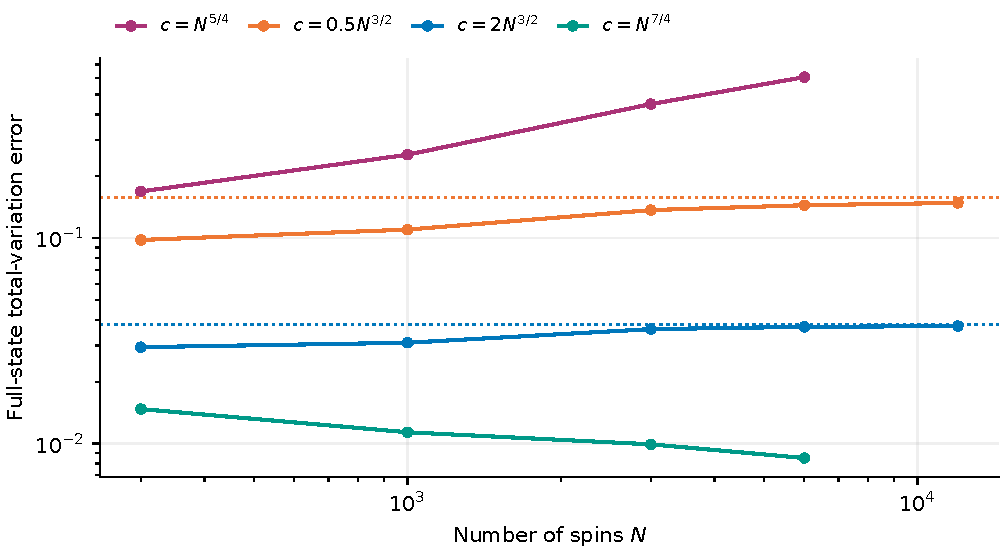
\includegraphics[width=.94\linewidth]{figures/potts-scaling.pdf}
 \caption{Exact finite-system mean-field Potts calculations with the
 physical secant bath. Points are occupation sums and Gamma/Beta CDF
 evaluations, connected to guide the eye. Dotted lines are the proved
 secant boundary limits for $c_N=\gamma N^{3/2}$, with
 $\gamma=0.5$ and $2$. The largest size, $N=12000$, was computed for
 these two boundary sequences; the other sequences extend to $N=6000$.
 These are mean-field data and do not test a short-range interfacial law.}
 \label{fig:potts-scaling}
\end{figure}

At $c_N=0.5N^{3/2}$ the predicted limit is approximately $0.157392$;
the exact $N=12000$ value is $0.148341$.
At $c_N=2N^{3/2}$ the corresponding values are $0.037986$ and
$0.037304$. These are secant-calibrated errors, not results of a
finite-$N$ optimization. The $N^{7/4}$ sequence illustrates decay
above the threshold; the $N^{5/4}$ sequence illustrates persistent
error below it. The finite range of sizes does not establish an
asymptotic exponent by itself. The theorem provides that conclusion.

These sizes are also far from the asymptotic regime of the phase
decomposition itself. The saddle of the rate function
\eqref{eq:mf-rate} at $(1/2,1/4,1/4)$ lies on the Voronoi boundary
between the ordered and disordered cells, and its rate excess is
$I(1/2,1/4,1/4)-I_{\min}=\log3-\tfrac{19}{12}\log2\simeq1.1\times10^{-3}$.
The interphase valley is therefore suppressed only by
$\exp(-0.0011N)$, which is of order one below $N\simeq10^3$.
Exact occupation sums for the pure-spin model show the slow approach.
Here Voronoi distance is Euclidean in the three occupation fractions;
ties between ordered and disordered cells are assigned to the ordered
phase. The combined ordered event is therefore $\max_j n_j\ge N/2$.
With this convention,
the Voronoi-conditional ordered variance divided by $N$ is
$1.02$ at $N=3000$ and $0.78$ at $N=12000$, against the limit
$v_-\simeq0.733$ from \eqref{eq:mf-variances}, while the ordered
weight is $0.528$ and $0.529$ against $w_-\simeq0.530$ from
\eqref{eq:mf-phase-weights}. The limiting formulas plotted as dotted
lines use the limiting constants; the finite-size points are exact.

Figure~\ref{fig:boundary-optimization} displays a different object:
the proved limiting formula for balanced phases of equal variance,
rather than microscopic finite-size enumeration.
Writing $\lambda=b\sqrt v$, preserving the phase weights gives
$2\Phi(\lambda/2)-1$, whereas optimizing the total energy gives
$\min\{2\Phi(\lambda/2)-1,1/2\}$.
The second branch is attained by abandoning one phase.
This example explains why an error report should include both the
TV value and the resulting phase populations.

\begin{figure}[t]
 \centering
 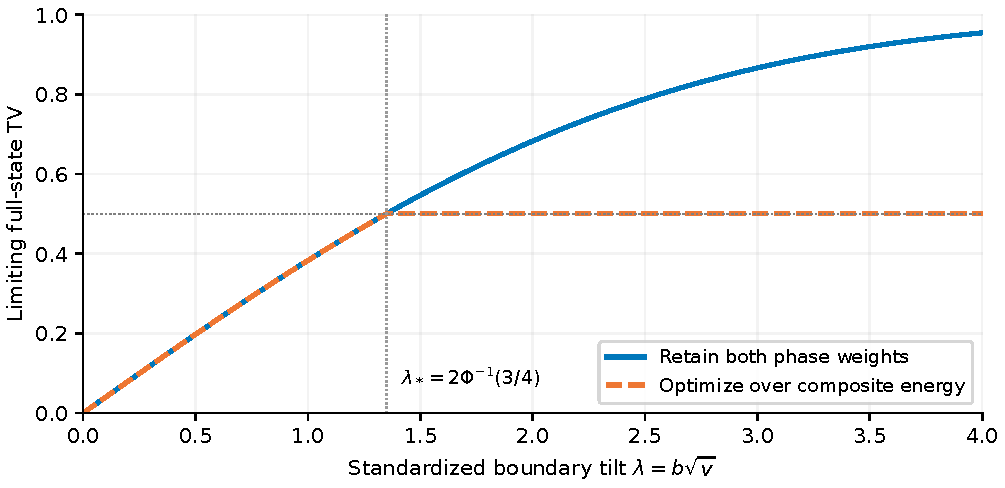
\includegraphics[width=.94\linewidth]{figures/boundary-optimization.pdf}
 \caption{The physical boundary law for balanced equal-variance phases
 under Theorem~\ref{thm:physical-boundary}'s moment and exceptional-mass
 hypotheses. This is an evaluation of the limiting formula, not
 finite-size Potts data. At
 $\lambda_*=2\Phi^{-1}(3/4)\simeq1.34898$, an optimizer that retains
 both phase populations and one that discards a phase have the same
 limiting error. The same curve holds for the exact scalar Gaussian
 model of Proposition~\ref{prop:scalar-gaussian}.}
 \label{fig:boundary-optimization}
\end{figure}

The accompanying source bundle retains the finite-system data,
figure code, and independent checks. Small systems are checked
against explicit enumeration of all $3^N$ labeled spin states for
$1\le N\le8$. At $N=12$, direct absolute-density integration verifies
the Gamma/Beta crossing formula for two kinetic shapes. Separate
normal-density quadratures verify the weighted CDF expression
\eqref{eq:physical-optimum-cdf} and its optimizer.
Floating-point calculations are numerical checks, not interval
certificates or substitutes for the proofs. The reproducibility
instructions distinguish quick checks and figure regeneration from
the more expensive full occupation enumeration through $N=12000$.

\section{Discussion and conclusions}
\label{sec:conclusions}

A reservoir requirement is precise only once we specify what must be
reproduced. The results separate three ingredients that are often
merged: the reservoir capacity, its calibration, and the observable
being tested. For the complete canonical law at coexistence, capacity
and calibration interact: the secant calibration removes the phase bias
caused by the latent heat, so the capacity needs to control only the
tilt within each phase. This is why two-phase coexistence needs $c_N\gg
N^{3/2}$ rather than the $N^2$ suggested by the latent heat or by the
subsystem's canonical heat capacity. Three distinct phase energies,
including the combined energy of two coexisting copies, restore the
$N^2$ requirement. Smooth reservoirs with positive heat capacity obey
the same curvature mechanism when a suitable calibration and tail
control are available. The heat-capacity convention also matters at
finite size, as finite ideal-gas contact calculations show
\cite{CortiEtAl2023}.

The observable matters as much. Phase weights should be reported with
any optimized error, since at the threshold scale the smallest
full-state TV can come from discarding a phase. Marginal and joint
accuracy differ: with balanced phase weights, a shared reservoir can
leave each copy canonical while anticorrelating their phases, an
equilibrium effect that needs no direct interaction between the copies.
Other criteria are not equivalent to full-state accuracy: a small
Euclidean histogram norm or macroscopic energy concentration does not
imply it, and the log-density barrier between a phase center and the
interphase midpoint can remain lowered by a large amount while the
full-state TV tends to zero.

The proved scope is equilibrium coupling to the stated reservoir with
additive energies, fixed positive limiting phase weights, and the
explicit fluctuation and tail hypotheses of each theorem. The
short-range results require a fixed number of colors $q\ge q_0(d)$.
Their threshold-scale law holds for every fixed capacity coefficient
$\gamma>0$ in dimensions above two, and for sufficiently large $\gamma$
in two dimensions. The square-torus interfacial calculation is a stated
capillarity model, not a derivation of microscopic droplet or slab
morphology, and the Gaussian, capillarity, and linear-capacity
appendices analyze stated models exactly, whereas the contour appendix
proves a microscopic hypothesis.

These limits suggest open questions: the two-dimensional threshold-scale
law for small $\gamma$, where interfacial configurations compete with
the phases; Potts models with fewer colors and other interacting
systems; interacting spatial subregions of a single system, which a
shared-reservoir model of independent copies does not describe; quantum
systems, in particular observables that do not commute with the energy;
and explicit finite-size error bounds.

\clearpage
\appendix
\section{Positive contour measures and the short-range theorem}
\label{app:short-range-proof}

This appendix proves Theorem~\ref{thm:sr-bath}. Its source estimates,
phase definitions, and energy observable are kept explicit because a
signed partition-function approximation alone does not control a
positive reweighted probability measure.

The color threshold $q_0(d)$ is fixed once, here. It is the largest of:
the thresholds required by the cited finite-size scaling and contour
results \cite{BorgsKoteckyMiracleSole1991,BorgsChayesTetali2012} on
a fixed temperature interval around coexistence; the value $2d+1$,
used for the variance lower bound in
\eqref{eq:sr-variance-lower}; and the value needed for the
cluster-expansion criterion of \cite{BorgsChayesTetali2012} to hold
with the extra factor $e^{\rho m_\gamma}$ in
\eqref{eq:sr-cluster-majorant} for a fixed $\rho>0$. Every
``sufficiently large $q$'' below refers to this single threshold.

\subsection{Published finite-volume inputs and normalization}

We use the following established contour results, with source locations
given so that the deductions can be distinguished from their inputs.
Theorem 1 of Borgs, Koteck\'y, and Miracle-Sol\'e~\cite{BorgsKoteckyMiracleSole1991}
gives six-times differentiable dimensionless free energies
$\psi_o,\psi_d$ and a fixed real interval containing $\beta_c$ on which
\begin{equation}
 Z_N^{\mathrm{spin}}(\beta)
 =q e^{-N\psi_o(\beta)}+e^{-N\psi_d(\beta)}
   +O(e^{-bL})e^{-N\min_i\psi_i(\beta)}.
 \label{eq:sr-partition-input}
\end{equation}
The constants are uniform on a sufficiently small fixed compact interval.
The source states its error as $O(q^{-bL})$; for fixed $q$ this is
$O(e^{-bL})$ with a different constant $b$, which is the form used here.
At coexistence the free energies are equal and
\begin{equation}
 u_i=\psi_i'(\beta_c),\qquad
 u_o<u_d,\qquad \sigma_i^2=-\psi_i''(\beta_c).
 \label{eq:sr-phase-parameters}
\end{equation}
The ordered branch is stable above $\beta_c$, and the disordered branch
below. The source Hamiltonian in its equation (6), with $J=1$, is exactly
\eqref{eq:sr-hamiltonian}. The notation here uses $\psi_i=\beta f_i$
relative to that source. No complex-temperature continuation of
\eqref{eq:sr-partition-input} is assumed.

For the positive decomposition, put $p=1-e^{-\beta}$ and use bond sets
$A\subseteq\mathcal B_L$. Their random-cluster weights are
\begin{equation}
 w_\beta(A)=p^{|A|}(1-p)^{dN-|A|}q^{k(A)},
 \qquad
 Z_N^{\mathrm{RC}}(\beta)=\sum_Aw_\beta(A)
 =e^{-\beta dN}Z_N^{\mathrm{spin}}(\beta).
 \label{eq:sr-rc-normalization}
\end{equation}
This normalization follows by expanding
$\prod_{\{x,y\}}[1+(e^\beta-1)\ind_{\{\sigma_x=\sigma_y\}}]$.
It fixes the additive energy convention independently of conventions
used in contour references.

Throughout the short-range proof, contours, interiors and exteriors,
compatibility, phase events, restricted partition functions, and activities
are those of Borgs, Chayes, and Tetali~\cite{BorgsChayesTetali2012}
(BCT), Definitions 4.1--4.4 and 5.4, equations (6.1)--(6.5) and
(6.13)--(6.22). In particular, BCT defines the exterior of a contour
as the component containing a compatible interface, if such an interface
exists; otherwise it chooses the larger component, with a fixed tie rule.
This convention matters for large contours on the torus.

Geometrically, the construction thickens the occupied bonds and separates
ordered and disordered regions by their boundary components. Components
with zero winding vector are contours; the remaining components are
interfaces. In the absence of interfaces, the common exterior of the
contours has one label, ordered or disordered, which defines the positive
event $\mathcal O_L$ or $\mathcal D_L$. Configurations with at least one
interface form the tunneling event $\mathcal T_L$. Thus these events
partition the bond configurations and are independent of $\beta$.
Let $Z_{o,L}$ denote the ordered contribution with its color
multiplicity removed, and $Z_{d,L}$ the disordered contribution. BCT
(6.1)--(6.5) give exactly
\begin{equation}
 Z_N^{\mathrm{RC}}=q Z_{o,L}+Z_{d,L}+Z_{t,L}.
 \label{eq:sr-positive-contour-decomposition}
\end{equation}
At $\beta_c$, BCT Lemma 6.1 bounds the tunneling probability by
$C e^{-bL^{d-1}}$. The later construction
in~\cite{BorgsChayesHelmuthPerkinsTetali2022}, Definition 5,
uses a modified exterior convention; we do not identify its finite-volume
phase events with those used here or import estimates between them.

We will use the following specific parts of the original contour
construction. Write $m_\gamma=\|\gamma\|$ for the contour size.
Its diameter obeys
\begin{equation}
 \operatorname{diam}\gamma\le L,\qquad
 \operatorname{diam}\gamma\le m_\gamma/2,\qquad
 |\operatorname{Int}\gamma\cap\Lambda_L|
       \le\tfrac12m_\gamma\operatorname{diam}\gamma.
 \label{eq:sr-contour-geometry}
\end{equation}
These are the definition of diameter and Lemma 5.7
of~\cite{BorgsChayesTetali2012}; they hold for all $d\ge2$.
The positive restricted partition functions have the polymer form
\begin{equation}
 Z_{i,L}=e^{-e_i(\beta)N}
       \sum_{\Gamma\ \mathrm{compatible}}
       \prod_{\gamma\in\Gamma}K_i(\gamma;\beta).
 \label{eq:sr-polymer-form}
\end{equation}
Here the explicit ground coefficients are
$e_o=-d\log(1-e^{-\beta})$, $e_d=d\beta-\log q$, and
$\kappa=\tfrac12\log(e^\beta-1)$.
The activities are $e^{-\kappa(\beta)m_\gamma}$ times a ratio of
positive interior partition functions, with a factor $q$ in the
disordered case; see equations (6.18)--(6.22) of that source. The
coefficients $e_i$ and $\kappa$ have bounded derivatives on the fixed
temperature interval considered here.

Appendix A defines truncated activities
\begin{equation}
 K_i'(\gamma;\beta)=\min\{K_i(\gamma;\beta),
                                  e^{-\tau(\beta)m_\gamma}\},
 \label{eq:sr-truncation}
\end{equation}
where BCT (A.3) uses $\tau(\beta)=\beta/8-\beta/20+1$.
This positive exponential cap ensures uniform convergence of the cluster
expansion when $q$ is sufficiently large. Its infinite-volume
free energies will be denoted $f_i^{\mathrm{tr}}$, to distinguish them
from the $\psi_i$ in~\eqref{eq:sr-partition-input}. If
$a_i=f_i^{\mathrm{tr}}-\min_j f_j^{\mathrm{tr}}$, Lemma A.1(i) states
\begin{equation}
 a_i(\beta)\operatorname{diam}\gamma\le c_0\beta
 \quad\Longrightarrow\quad K_i(\gamma;\beta)=K_i'(\gamma;\beta).
 \label{eq:sr-inactive-cutoff-input}
\end{equation}
Moreover, equation (A.8) on the full torus gives
\begin{equation}
 |\log Z_{i,L}'(\beta)+Nf_i^{\mathrm{tr}}(\beta)|
       \le CNe^{-bL}.
 \label{eq:sr-truncated-volume-input}
\end{equation}
The assumptions of Appendix A cover a fixed neighborhood on both sides
of $\beta_c$, even though the main-text Lemma 6.3 is stated on the
ordered side. To identify the stable sides within this same construction, BCT
Lemma A.3 says that the spontaneous magnetization is positive exactly
when $a_o=0$. BCT define their transition point $\beta_0$ as the onset
of positive magnetization, whereas $\beta_c$ above is the crossing
$\psi_o=\psi_d$ of the BKMS free energies. The two coincide: for
$q\ge q_0(d)$ the model has a unique, disordered Gibbs state below the
large-$q$ transition point and $q$ ordered extremal states above it
\cite{KoteckyShlosman1982,LaanaitEtAl1991}, and the BKMS expansion
\eqref{eq:sr-partition-input} is derived from the same Pirogov--Sinai
construction, in which the phase with the smaller $\psi_i$ is the
stable one at each $\beta$. Hence the magnetization vanishes below
$\beta_c$ and is positive above it, so $a_d=0$ below and $a_o=0$
above. Continuity gives $f_o^{\mathrm{tr}}=f_d^{\mathrm{tr}}$ at
coexistence.

The minimum $f^{\mathrm{tr}}=\min_i f_i^{\mathrm{tr}}$ is the physical
thermodynamic random-cluster free energy. This identification can be made
directly in the original convention: BCT Lemma A.1(ii), on the full torus,
bounds each $Z_{i,L}$ above by
$\exp[-Nf^{\mathrm{tr}}+O(Ne^{-bL})]$, while (A.9) supplies the
corresponding lower bound for any minimizing phase. The interface-network
sum (6.26)--(6.27) bounds $Z_{t,L}$ by
$\exp[-Nf^{\mathrm{tr}}-bL^{d-1}]$.
That sum uses only the bounds from Appendix A and the large-$q$ contour
counting inequalities, which hold throughout the fixed neighborhood
under consideration; shrink the neighborhood if necessary so that
$q\le e^{2d\kappa+d}$ there, as required in (6.27).
The sum does not require the ordered phase to minimize.
Combining these estimates with
\eqref{eq:sr-positive-contour-decomposition} identifies the limiting
pressure. Equation~\eqref{eq:sr-rc-normalization} and the stable branch
of~\eqref{eq:sr-partition-input} consequently give
\begin{equation}
 f_i^{\mathrm{tr}}(\beta)=\psi_i(\beta)+d\beta
 \quad\text{on the stable side of phase }i.
 \label{eq:sr-stable-branch-identification}
\end{equation}
We do not identify the two metastable constructions away from their
stable sides or assume differentiability of the minimum cutoff.

\subsection{Weak phase energy limits and nonzero variances}

Applying~\eqref{eq:sr-partition-input} at $\beta_c+t/N$ and using the
boundedness of $U_N/N$ gives
\begin{equation}
 U_N/N\ \Rightarrow\ \frac q{q+1}\delta_{u_o}
                           +\frac1{q+1}\delta_{u_d}.
 \label{eq:sr-macro-limit}
\end{equation}
Indeed the ratios of partition functions are Laplace transforms and
converge for every fixed real $t$ to those of the displayed bounded law.
Define the actual spin events
$B_{o,N}=\{U_N/N<(u_o+u_d)/2\}$ and $B_{d,N}=B_{o,N}^c$.
Their limiting probabilities are the two weights in
\eqref{eq:sr-macro-limit}.

For $s>0$, use~\eqref{eq:sr-partition-input} at
$\beta_c+s/\sqrt N$. The ordered branch dominates, and its quadratic
Taylor expansion gives
\begin{equation}
 \E_{\beta_c}\exp[-s(U_N-Nu_o)/\sqrt N]
       \longrightarrow\frac q{q+1}e^{\sigma_o^2s^2/2}.
 \label{eq:sr-one-sided-laplace}
\end{equation}
The part on $B_{d,N}$ is at most
$e^{-s(u_d-u_o)\sqrt N/2}$ and vanishes. Thus this is also the transform
limit of the positive subprobability measure restricted to $B_{o,N}$.
The disordered phase uses the opposite sign and $\beta_c-s/\sqrt N$.

For clarity, a one-sided transform limit suffices here. Tilt the ordered
subprobability law of $x=(U_N-Nu_o)/\sqrt N$ by $e^{-s_0x}$ for any
fixed $s_0>0$ and normalize it. Ratios of
\eqref{eq:sr-one-sided-laplace} at $s_0-t$ and $s_0$, for $|t|<s_0$,
give convergence of its moment-generating function to that of
$\Normal(-\sigma_o^2s_0,\sigma_o^2)$. The ordinary moment-generating
function convergence theorem gives weak convergence of these tilted
probabilities. Untilting against compactly supported continuous functions
gives vague convergence of the original positive measures. Their known
total masses converge to the recovered Gaussian mass, so vague convergence
is weak convergence. Hence
\begin{equation}
 (U_N-Nu_i)/\sqrt N\mid B_{i,N}
       \Rightarrow\Normal(0,\sigma_i^2),\qquad i=o,d.
 \label{eq:sr-conditional-clt}
\end{equation}
The variance is initially allowed to be zero; nonnegativity follows from
convexity of the limiting log transforms.

Both variances are in fact strictly positive. Here the requirement
$q>2d$ in the choice of $q_0(d)$ is used. Choose an independent
vertex set $S$ of size at least $N/(2d+1)$ and condition on all spins
outside it. The remaining spins are independent. For $x\in S$, let
$n_{x,a}$ count the neighbors of color $a$. Then
$\sum_a n_{x,a}=2d$, and the conditional color probabilities on a
compact inverse-temperature interval with upper endpoint $\beta_{\max}$
obey $p_{x,a}\ge q^{-1}e^{-2d\beta_{\max}}$. If $q>2d$, two neighbor
counts differ by at least one. Since
$\Var_p(n)=\sum_{a<b}p_ap_b(n_a-n_b)^2$, conditional variance gives
\begin{equation}
 \Var_\beta U_N\ge v_*N,\qquad
 v_*:=\frac{e^{-4d\beta_{\max}}}{(2d+1)q^2}>0.
 \label{eq:sr-variance-lower}
\end{equation}
Thus $N^{-1}\log Z_N^{\mathrm{spin}}-v_*\beta^2/2$ is convex.
Its pointwise thermodynamic limit is convex as well. On each open stable
side that limit equals $-\psi_i(\beta)-v_*\beta^2/2$, so
$-\psi_i''\ge v_*$. Continuity of $\psi_i''$ extends the bound to
$\beta_c$, proving $\sigma_i^2\ge v_*>0$. This argument passes through
the stable thermodynamic branches; it does not infer a phase variance
from the much larger total coexistence variance.

\subsection{Uniform moments from positive contour measures}
\label{subsubsec:sr-moments}

We next establish the inward fluctuation control needed for sufficiency.
The finite-volume argument is useful because the minimum in
\eqref{eq:sr-truncation} need not be twice differentiable. The proof
requires only a Lipschitz estimate for its limiting free energy and
then removes every cutoff in a small real temperature interval.

\begin{lemma}[Restricted contour partition derivatives]
\label{lem:sr-restricted-derivatives}
For the fixed sufficiently large $q$ above, there are constants
$\eta,C>0$ such that, for $i=o,d$ and all sufficiently large $L$,
\begin{equation}
 \left|\frac{\dd^2}{\dd\beta^2}\log Z_{i,L}(\beta)\right|\le CN,
 \qquad |\beta-\beta_c|\le\eta/L.
 \label{eq:sr-restricted-second}
\end{equation}
On this interval $Z_{i,L}=Z_{i,L}'$, and
\begin{equation}
 \left.\frac{\dd}{\dd\beta}
 \log[e^{d\beta N}Z_{i,L}(\beta)]\right|_{\beta=\beta_c}
       =-Nu_i+O(\sqrt N).
 \label{eq:sr-restricted-center}
\end{equation}
\end{lemma}
\begin{proof}
We supply the derivative bounds underlying the use of the cluster
expansion. For a general contour interior $\Lambda=\operatorname{Int}\gamma$,
use the positive matching-label sums in BCT (6.13)--(6.14). A summand
indexed by an admissible family $\Gamma$ has logarithm
\begin{equation}
 F_\Gamma(\beta)
 =-e_o(\beta)n_o(\Gamma)-e_d(\beta)n_d(\Gamma)
   -\kappa(\beta)M(\Gamma)+c_\Gamma\log q,
 \label{eq:sr-matching-summand}
\end{equation}
where $n_o+n_d=|\Lambda\cap\Lambda_L|$, the nonnegative integers
$n_o,n_d$ count vertices with each label, and
$M(\Gamma)=\sum_{\gamma'\in\Gamma}m_{\gamma'}$ counts internal contour
intersections. The integer $c_\Gamma$ counts ordered components, with
the constant subtraction of one when the ordered color multiplicity is
removed. All these quantities and the set of admissible families are
independent of $\beta$.

To bound $M(\Gamma)$, recall BCT's construction from cubes of side
$1/2$ and its definition of contour size as the number of
intersections with lattice edges, Section 4 and equation (4.5).
Each contour surface is a union of faces of the half-integer cube
lattice, so it meets a given lattice edge in at most a fixed number
$C_d'$ of points, and pairwise compatible contours are disjoint, so
the intersections counted by $M(\Gamma)$ are distinct points on
distinct edges or on distinct contours. A contour of $\Gamma$ lies in
the closure of $\Lambda$, so the edges it meets either have an
endpoint in $\Lambda\cap\Lambda_L$, of which there are at most
$2d|\Lambda\cap\Lambda_L|$, or cross the bounding contour $\gamma$,
of which there are at most $m_\gamma$ by the definition of contour
size. Consequently
\[
 M(\Gamma)\le C_d'\bigl(2d|\Lambda\cap\Lambda_L|+m_\gamma\bigr)
 \le C_d\bigl(|\Lambda\cap\Lambda_L|+m_\gamma\bigr)
 =:C_d V_\gamma.
\]
The bounded derivatives of $e_o,e_d,\kappa$ now give
$|F_\Gamma'|+|F_\Gamma''|\le C V_\gamma$.
This argument applies to the matching-label sums even when the interior
wraps around the torus; it requires no interpretation as an unrestricted
random-cluster partition function on a simply connected region.

For a positive sum $S=\sum_\Gamma e^{F_\Gamma}$, direct differentiation gives
\[
 (\log S)'=\E_S F_\Gamma',\qquad
 (\log S)''=\E_S F_\Gamma''+\Var_S F_\Gamma'.
\]
Hence $|(\log S)'|\le CV_\gamma$ and
$|(\log S)''|\le C(V_\gamma+V_\gamma^2)$.
Apply these bounds to the numerator and denominator in BCT's activity
ratios (6.18) and (6.22). Since
$V_\gamma=O(m_\gamma^2)$ by~\eqref{eq:sr-contour-geometry}, this
gives the uniform real-parameter bounds
\begin{equation}
 |\partial_\beta\log K_i(\gamma)|\le Cm_\gamma^2,
 \qquad
 |\partial_\beta^2K_i(\gamma)|
                \le Cm_\gamma^4K_i(\gamma).
 \label{eq:sr-activity-derivatives}
\end{equation}
These inequalities do not require the interior phase to be stable.

Here are the precise summability estimates used to differentiate.
For a cluster $\mathcal C$, write
$m(\mathcal C)=\sum_{\gamma\in\mathcal C}m_\gamma$ and let
$\Phi(\mathcal C)$ denote its Ursell coefficient, including the
factor for repeated polymers. The contour counting and incompatibility
estimates (A.5)--(A.6) of~\cite{BorgsChayesTetali2012} give, for some fixed $\rho>0$,
\begin{equation}
 \sum_{\mathcal C}|\Phi(\mathcal C)|
       \prod_{\gamma\in\mathcal C}K_i'(\gamma;\beta)
       e^{\rho m(\mathcal C)}\le CN.
 \label{eq:sr-cluster-majorant}
\end{equation}
The factor $e^{\rho m_\gamma}$ is absorbed by the choice of
$q_0(d)$: the criterion (A.5)--(A.6) holds with a slack
$e^{(c\beta+1)m_\gamma}$ that grows with $q$, so a fixed
$\rho<c\beta+1$ leaves the criterion satisfied on the temperature
interval. To sum over clusters, use the device of BCT's proof of
Lemma A.2 (their Appendix A.3): every contour in $\Lambda_L$ is
incompatible with at least one of the $N$ contours of size two
obtained from configurations with a single disordered edge in a
fixed direction. Every cluster therefore contains a contour
incompatible with one of these $N$ fixed contours, and summing the
incompatibility bound (A.6) over them, with the polynomial factor
absorbed in the exponential slack, proves
\eqref{eq:sr-cluster-majorant}. Overcounting clusters that are
incompatible with several fixed contours only increases the upper
bound.

On any compact real temperature interval, the minimum in
\eqref{eq:sr-truncation} is absolutely continuous. Almost everywhere,
its logarithmic derivative is that of one of its two positive branches;
both obey $|\partial_\beta K_i'|\le Cm_\gamma^2K_i'$.
Termwise first differentiation is therefore justified by
\eqref{eq:sr-cluster-majorant}, since a differentiated cluster is bounded
by $C m(\mathcal C)^2$ times its absolute weight. Equivalently, integrate
these almost-everywhere derivatives over the parameter interval and use
the same majorant to interchange sum and integral. Including the ground
term in~\eqref{eq:sr-polymer-form} gives
$|\partial_\beta\log Z_{i,L}'|\le CN$ almost everywhere. Hence the
finite-volume free energies are uniformly Lipschitz. Their pointwise
limits $f_i^{\mathrm{tr}}$ are Lipschitz with the same constant.

Since $a_i(\beta_c)=0$ and $a_i$ is the difference of two functions
with Lipschitz constant $C$, it follows that
$a_i(\beta)\le 2C|\beta-\beta_c|$. Choose $\eta>0$ small enough that
$2C\eta<c_0\inf\beta$ on the fixed interval. Every torus contour has
diameter at most $L$, so~\eqref{eq:sr-inactive-cutoff-input} now removes
\emph{all} cutoffs on $|\beta-\beta_c|\le\eta/L$.
The finite-volume activities on this interval are their original smooth
positive functions. A second derivative of a cluster product is bounded
by $C m(\mathcal C)^4$ times its absolute weight, by
\eqref{eq:sr-activity-derivatives}. The exponential factor in
\eqref{eq:sr-cluster-majorant} absorbs this polynomial uniformly.
Twice differentiating the uniformly convergent cluster expansion,
and adding the ground term, proves~\eqref{eq:sr-restricted-second}.
This step differentiates no minimum cutoff.

For the center, set
$F_{i,L}(\beta)=\log[e^{d\beta N}Z_{i,L}(\beta)]$ and take
$t_N=\eta/(2\sqrt N)$ with the sign pointing to the stable side of
phase $i$. Since $d\ge2$, $|t_N|\le\eta/L$. Equations
\eqref{eq:sr-truncated-volume-input} and
\eqref{eq:sr-stable-branch-identification} give, both at $\beta_c$ and
at $\beta_c+t_N$,
$F_{i,L}(\beta)=-N\psi_i(\beta)+O(Ne^{-bL})$.
The second-derivative bound and a stable-side finite difference imply
\[
 F_{i,L}'(\beta_c)
 =-N\frac{\psi_i(\beta_c+t_N)-\psi_i(\beta_c)}{t_N}
     +O(N|t_N|)+O(Ne^{-bL}/|t_N|)
 =-Nu_i+O(\sqrt N).
\]
The exponentially small error is negligible for fixed $d$, proving
\eqref{eq:sr-restricted-center}.
\end{proof}

\begin{lemma}[Transfer from bond fluctuations to spin energy]
\label{lem:sr-energy-transfer}
In the Edwards--Sokal joint law at $\beta_c$, the conditional spin
energy on each of the positive bond phase events obeys
\begin{equation}
 \sup_{L\ge L_0,i\in\{o,d\}}
 \E\left[\exp\left(\eta_1\frac{|U_N-Nu_i|}{\sqrt N}\right)
                 \,\middle|\,\mathcal I_{i,L}\right]<\infty
 \label{eq:sr-spin-phase-moment}
\end{equation}
for some fixed $\eta_1>0$ and sufficiently large fixed $L_0$, where
$\mathcal I_{o,L}=\mathcal O_L$ and
$\mathcal I_{d,L}=\mathcal D_L$.
\end{lemma}
\begin{proof}
Introduce the bond fugacity parameter $\lambda=\log(e^\beta-1)$;
then $\dd\beta/\dd\lambda=p$. Put $B=|A|$ and
$M=-U_N$, the number of monochromatic spin bonds. The partition
function $e^{d\beta N}Z_{i,L}(\beta)$ is, up to the constant ordered
multiplicity, a positive sum of $e^{\lambda B}q^{k(A)}$ over the fixed
phase event. Therefore the first and second derivatives of its
\emph{logarithm},
$F_{i,L}(\beta)=\log[e^{d\beta N}Z_{i,L}(\beta)]$, with respect to
$\lambda$ are the conditional mean and variance of $B$.

Lemma~\ref{lem:sr-restricted-derivatives}, the bounded derivatives of
$\beta(\lambda)$, and the elementary $|F_{i,L}'|\le CN$ give a second
$\lambda$ derivative bounded by $CN$ throughout a window of width
$\eta_2/\sqrt N$. At coexistence the first derivative is
$-pNu_i+O(\sqrt N)$, by~\eqref{eq:sr-restricted-center}.
Taylor's theorem for log partition ratios at
$\lambda_c\pm\eta_3/\sqrt N$ therefore proves
\begin{equation}
 \E\left[e^{\eta_3|B+pNu_i|/\sqrt N}
                     \,\middle|\,\mathcal I_{i,L}\right]\le C
 \label{eq:sr-bond-moment}
\end{equation}
for a sufficiently small fixed $\eta_3>0$.

Conditional on the spin configuration, $B$ is Binomial$(M,p)$, since
each monochromatic bond is retained independently with probability $p$.
For a centered Bernoulli variable, the second derivative of its log
moment-generating function is at most $1/4$; integrating twice bounds
that function by $t^2/8$. Conditional independence therefore gives,
for $D=B-pM$,
\begin{equation}
 \E[e^{tD}\mid\sigma]\le e^{dNt^2/8}
 \quad(t\in\R),\qquad
 \E e^{t|D|/\sqrt N}\le2e^{dt^2/8}.
 \label{eq:sr-binomial-noise}
\end{equation}
This estimate remains bounded after conditioning on any event whose
probability is bounded below, at the cost of dividing by that probability.
At coexistence all cutoffs are inactive, and
\eqref{eq:sr-truncated-volume-input} with equal free energies, together
with the tunneling bound, gives
\begin{equation}
 P(\mathcal O_L)\to\frac q{q+1},\qquad
 P(\mathcal D_L)\to\frac1{q+1},\qquad
 P(\mathcal T_L)\le Ce^{-bL^{d-1}}.
 \label{eq:sr-positive-phase-probabilities}
\end{equation}
Thus the conditional noise moments are uniformly bounded. Finally
\[
 |U_N-Nu_i|=|M+Nu_i|
 \le p^{-1}\{|B+pNu_i|+|D|\}.
\]
Cauchy--Schwarz,~\eqref{eq:sr-bond-moment}, and
\eqref{eq:sr-binomial-noise} prove~\eqref{eq:sr-spin-phase-moment}
with $2\eta_1/p\le\eta_3$.
\end{proof}

This transfer uses a conditional binomial fluctuation estimate, not an
identification of occupied bonds with spin energy. In particular,
differentiating the restricted bond partition function gives the bond
count first; the noise estimate is the additional step needed for the
physical Hamiltonian.

\begin{proof}[Proof of Theorem~\ref{thm:sr-bath}]
For necessity, the positive midpoint phase weights,
\eqref{eq:sr-conditional-clt}, and $\sigma_i^2\ge v_*>0$ satisfy
Theorem~\ref{thm:two-scale-necessity}, with gap $N(u_d-u_o)$ and
$s_N=\sqrt N$.

For sufficiency, use the positive decomposition by
$\mathcal O_L,\mathcal D_L,\mathcal T_L$ on the Edwards--Sokal space.
Lemma~\ref{lem:sr-energy-transfer} supplies the physical-energy moment
bound. The exceptional mass is at most $Ce^{-bL^{d-1}}$, while the
largest bath amplification is $\exp[O(N^2/c_N)]$. If
$c_N\gg N^{3/2}$, its logarithm is $o(\sqrt N)=o(L^{d/2})$.
Since $d-1\ge d/2$ for $d\ge2$, the exceptional contribution vanishes.
Theorem~\ref{thm:positive-sufficiency} therefore gives total-variation
convergence on the joint spin--bond space. The likelihood there is
the exact function of $U_N(\sigma)$ in~\eqref{eq:exact-marginal}.
Summing over bonds gives precisely the physical subsystem law, so
projection proves the claimed spin conclusion.
\end{proof}

The argument establishes a small fixed exponential moment on the
$\sqrt N$ scale. It neither asserts a global Gaussian phase tail nor
requires one. Optional independent quadratic momenta preserve the
threshold: their centered Gamma transform adds the moment bound from
Lemma~\ref{lem:mf-exponential}, their mean shifts both centers by
$aN/\beta_c$, and their variance adds $a/\beta_c^2$ to the weak phase
limits. For $a>0$ convolution also yields continuous local Gaussian
energy limits, but no short-range pointwise density envelope is needed
for Theorem~\ref{thm:sr-bath}.

\section{Exact Gaussian models and calibration geometry}
\label{sec:gaussian-geometry}

Gaussian reservoirs and Gaussian descriptions of homogeneous coexistence
peaks have a substantial history~\cite{ChallaHetherington1988PRL,ChallaLandauBinder1986}.
Here they are exact probability models used to isolate calibration and
phase-selection effects. Their interphase tails are not substituted for
the microscopic laws of Section~\ref{sec:microscopic}. A quadratic
residual weight also differs from the exact power-law reservoir: the
identification $\kappa=\beta^2/(C_B/k_B)$ describes a local entropy curvature,
not a globally constant heat capacity for an exactly quadratic entropy.

\subsection{Two scalar phases and the optimized error crossover}

Let $\varphi_{s^2}$ denote a centered normal density with standard
deviation $s>0$, and consider
\begin{equation}
 p_N(E)=\tfrac12\varphi_{s_N^2}(E-m_N)+\tfrac12\varphi_{s_N^2}(E+m_N),
 \quad m_N/s_N\to\infty,
 \qquad
 q_{N,t}\propto p_N e^{tE-\kappa_NE^2/2},\quad\kappa_N\ge0.
 \label{eq:scalar-gaussian-model}
\end{equation}
The field $t\in\R$ is unrestricted. Completion of squares gives the
transformed component variance, means, and upper-phase weight:
\begin{equation}
 \widetilde s_N^2=\frac{s_N^2}{1+\kappa_Ns_N^2},\qquad
 \widetilde m_{\pm,N}=\frac{\pm m_N+t s_N^2}{1+\kappa_Ns_N^2},\qquad
 v_{+,N}(t)=\frac1{1+e^{-2tm_N/(1+\kappa_Ns_N^2)}}.
 \label{eq:scalar-gaussian-completion}
\end{equation}

\begin{proposition}[Scalar convergence and optimized crossover]
\label{prop:scalar-gaussian}
There exists a field sequence giving $\TV(p_N,q_{N,t_N})\to0$ if and
only if $\kappa_Nm_Ns_N\to0$. If instead
$\kappa_Nm_Ns_N\to a\in[0,\infty)$, then
\begin{align}
 \TV(p_N,q_{N,0})&\longrightarrow2\Phi(a/2)-1,
 \label{eq:scalar-balanced-crossover}\\
 \inf_{t\in\R}\TV(p_N,q_{N,t})
       &\longrightarrow\min\{2\Phi(a/2)-1,1/2\}.
 \label{eq:scalar-optimal-crossover}
\end{align}
\end{proposition}
\begin{proof}
Put $r_N=m_N/s_N$, $k_N=\kappa_Ns_N^2$, and $b_N=t_Ns_N$.
In units of $s_N$, the transformed means are
$(\pm r_N+b_N)/(1+k_N)$ and their variance is $(1+k_N)^{-1}$.
If $\kappa_Nm_Ns_N\to0$, then $k_N\to0$ and the choice $t_N=0$
preserves the weights exactly while making both standardized mean
displacements vanish. Componentwise Gaussian TV convergence proves
sufficiency.

For necessity, we use the scalar case of the label-matching argument
given in full for Theorem~\ref{thm:gaussian-geometry}. Fix $R>0$ and
take the windows $|E\mp m_N|\le Rs_N$. Each has target mass tending to
$\tfrac12[2\Phi(R)-1]$, and the windows are disjoint for large $N$.
A transformed component has standard deviation
$\widetilde s_N\le s_N$, so the smaller of its probabilities in
these two windows tends to zero as $m_N/s_N\to\infty$.
TV convergence therefore forces both
components to keep weights with lower limit at least
$\tfrac12[2\Phi(R)-1]$, each supplying one window, and
letting $R\to\infty$ gives weights tending to $1/2$ and centers
$\widetilde m_{\pm,N}=\pm m_N+O(s_N)$, matched in their natural
order. Subtracting these center estimates and using the exact
transformed means gives
\[
 \frac{2r_N}{1+k_N}=2r_N+O(1),\qquad
 \frac{k_Nr_N}{1+k_N}=O(1).
\]
Since $r_N\to\infty$, this forces $k_N\to0$, so the variance ratio
already tends to one. Restricting to the matched windows and then
letting $R\to\infty$ gives TV convergence of each transformed
component to its target normal. In particular, its probability above
the target mean tends to $1/2$. With standardized displacement
$\delta_{\pm,N}=(b_N\mp k_Nr_N)/(1+k_N)$, this probability is
$\Phi(\delta_{\pm,N}\sqrt{1+k_N})$. Hence both displacements tend
to zero. Subtracting them proves $k_Nr_N\to0$.

For the finite crossover, $k_N\to0$ follows already from $k_Nr_N\to a$
and $r_N\to\infty$. At $t_N=0$ the two translated limiting normals
have displacements $\mp a$ and unit variance. Separating their windows
gives~\eqref{eq:scalar-balanced-crossover}, using
$\TV(\Normal(0,1),\Normal(a,1))=2\Phi(|a|/2)-1$.

To optimize, take any sequence of fields and a subsequence on which
the transformed upper weight converges. If its limit lies strictly
between zero and one, the logistic formula in
\eqref{eq:scalar-gaussian-completion} implies $b_N=O(1/r_N)$.
The limiting component displacements are therefore still $\mp a$.
The limiting TV is a convex function of the limiting upper weight,
and reflection makes that function symmetric about $1/2$. It is
minimized there, giving the first term in~\eqref{eq:scalar-optimal-crossover}.
If one weight tends to zero, a single bounded-width Gaussian cannot
cover both target windows, so the limiting lower bound is $1/2$.
This also covers means that escape all target windows. These subsequence
bounds apply to arbitrary approximate minimizers of the infimum.
The balanced choice attains the first bound. For $a>0$, the choice
$t_N=\kappa_Nm_N$ centers the upper component exactly at $m_N$, makes
its weight tend to one, and attains $1/2$. If $a=0$, the balanced bound
already vanishes.
\end{proof}

The optimizer changes behavior at
$a_*=2\Phi^{-1}(3/4)\simeq1.34898$. Above this value the TV objective
can favor an accurate single phase while discarding the other one.
An optimized scalar distance should therefore be accompanied by the
phase probabilities.

Temperature calibration changes the required scale even within this
simple model. Give the upper reference phase weight $w\ne1/2$, with
$0<w<1$, and hold the tangent of the quadratic bath at the canonical
mean $\bar E_N=(2w-1)m_N$. This means
$q_N\propto p_Ne^{-\kappa_N(E-\bar E_N)^2/2}$, or
$t_N=\kappa_N\bar E_N$. The exact transformed phase odds are
\begin{equation}
 \log\frac{v_{+,N}}{1-v_{+,N}}
 =\log\frac w{1-w}
   +\frac{2\kappa_N(2w-1)m_N^2}{1+\kappa_Ns_N^2}.
 \label{eq:gaussian-untuned-odds}
\end{equation}
The same separated-window argument first requires
$\kappa_Ns_N^2\to0$; convergence of the weights then requires
$\kappa_Nm_N^2\to0$. Conversely, that condition makes both the weight
and shape errors vanish. Thus for $m_N\asymp N$, $s_N\asymp\sqrt N$,
this specified untuned prescription requires $\kappa_NN^2\to0$,
whereas an appropriately tuned two-phase law needs only
$\kappa_NN^{3/2}\to0$. The reference point in this comparison is fixed
by the target canonical mean, not by a self-consistent modified mean.

\subsection{Several exchanged quantities and phase geometry}

Let the Gaussian variable be $Y\in\R^d$, where here $d$ is the number
of exchanged quantities, not a spatial dimension. Fix distinct phase
points $e_1,\ldots,e_k$ and positive weights $w_i$ summing to one. Set
\begin{equation}
 p_N=\sum_{i=1}^k w_i\Normal(Ne_i,NI_d),\qquad
 q_{N,t}\propto p_N\exp(t\cdot Y-\kappa_N|Y|^2/2),
 \quad t\in\R^d,\quad\kappa_N\ge0.
 \label{eq:multivariate-gaussian-model}
\end{equation}
With
\begin{equation}
 s_N=(1+\kappa_NN)^{-1},\qquad
 \alpha_N=\frac{\kappa_NN^2}{1+\kappa_NN},\qquad
 z_N=\frac{Nt}{1+\kappa_NN},
 \label{eq:multivariate-parameters}
\end{equation}
the transformed covariance is $Ns_NI_d$, its means are $Ns_N(e_i+t)$,
and its weights are
\begin{equation}
 v_{i,N}=\frac{w_i\exp(z_N\cdot e_i-\alpha_N|e_i|^2/2)}
                 {\sum_jw_j\exp(z_N\cdot e_j-\alpha_N|e_j|^2/2)}.
 \label{eq:multivariate-weights}
\end{equation}
For any affine dependence $(a_1,\ldots,a_k)$, meaning
$\sum_i a_i=0$ and $\sum_i a_ie_i=0$, this gives the exact invariant
\begin{equation}
 \sum_i a_i\log(v_{i,N}/w_i)
       =-\frac{\alpha_N}{2}\sum_i a_i|e_i|^2.
 \label{eq:multivariate-invariant}
\end{equation}
Every adjustable field has canceled.

\begin{theorem}[Geometry of Gaussian reservoir convergence]
\label{thm:gaussian-geometry}
For $k\ge2$, some field sequence in
\eqref{eq:multivariate-gaussian-model} gives TV convergence if and only if
\begin{equation}
 \begin{cases}
 \kappa_NN^{3/2}\to0,&\text{if the phase points are cospherical},\\
 \kappa_NN^2\to0,&\text{otherwise}.
 \end{cases}
 \label{eq:gaussian-geometry-classification}
\end{equation}
For $k=1$, the condition is $\kappa_NN\to0$. Cospherical means
that the points lie on a common sphere of positive radius in $\R^d$;
in $d=1$ a sphere is a pair of points, so three distinct scalar
phase points are never cospherical.
\end{theorem}
\begin{proof}
First justify matching the component labels. On the macroscopic
variable $Y/N$, every transformed covariance is at most $I_d/N$.
If TV tends to zero, each target phase neighborhood of positive mass
must therefore receive a distinct transformed component of nonvanishing
weight. There are exactly $k$ components, so this is a bijection, and
the matched transformed centers $s_N(e_i+t_N)$ lie in bounded
neighborhoods of the phase points; in particular they are bounded.
Along any subsequence, take a
further subsequence on which $s_N$, the translation $s_Nt_N$, and the
matching permutation converge. The limiting map $e\mapsto se+a$
maps the finite phase set onto itself. Its positive diameter forces
$s=1$, and the arithmetic centroid then forces $a=0$. Distinct phase
points make the matching permutation the identity. It follows that
$s_N\to1$, $s_Nt_N\to0$, and $v_{i,N}\to w_i$ with the original labels.

Isolating each matched component in expanding fluctuation windows
then gives its Gaussian TV convergence. In particular,
\begin{equation}
 \sqrt N\{(s_N-1)e_i+s_Nt_N\}\longrightarrow0
 \quad\hbox{for every }i.
 \label{eq:gaussian-shape-necessity}
\end{equation}
This necessity can also be detected by projection onto the direction
of a component's mean displacement. Subtracting two equations in
\eqref{eq:gaussian-shape-necessity} proves
$\kappa_NN^{3/2}\to0$ for any two distinct phase points.

The phase-weight equations $v_i=w_i$, when $\alpha_N>0$, are solvable
exactly if and only if
\begin{equation}
 |e_i|^2=2c\cdot e_i+b\quad\hbox{for every }i
 \label{eq:cosphere-equation}
\end{equation}
for some $c\in\R^d,b\in\R$. This is the sphere condition. Taking
$t_N=\kappa_NNc$ then restores every weight exactly and makes the
standardized mean changes
$\kappa_NN^{3/2}(c-e_i)/(1+\kappa_NN)$ tend to zero. This proves
sufficiency in the spherical case.

If~\eqref{eq:cosphere-equation} has no solution, finite-dimensional
linear algebra gives an affine dependence with
$\sum_i a_i|e_i|^2\ne0$. Since $v_{i,N}/w_i\to1$,
\eqref{eq:multivariate-invariant} forces $\alpha_N\to0$, equivalent
to $\kappa_NN^2\to0$. Taking $t_N=0$ proves sufficiency, including
the component shapes. For a single phase, $t_N=\kappa_NNe_1$ aligns
its mean exactly; matching the covariance is equivalent to
$\kappa_NN\to0$ and is necessary whatever mean is chosen.
\end{proof}

Every affinely independent set of at most $d+1$ points is cospherical,
but larger sets may also be cospherical. The number of phases alone
therefore does not determine the threshold in this vector model.
For scalar phase points $-1,0,1$, the invariant reads
\begin{equation}
 \frac{v_{+,N}v_{-,N}}{v_{0,N}^2}
       =\frac{w_+w_-}{w_0^2}e^{-\alpha_N}.
 \label{eq:three-gaussian-invariant}
\end{equation}
Three distinct scalar points are not cospherical, so their threshold
is $\kappa_NN^2\to0$.

\subsection{The exact optimum when some phases must disappear}

An empty-sphere contact set is a nonempty subset of phase indices of
the form
\begin{equation}
 F(c)=\operatorname*{arg\,min}_{1\le i\le k}|e_i-c|^2,
 \qquad c\in\R^d.
 \label{eq:empty-sphere-contact}
\end{equation}
These are the contact sets of the usual lower-paraboloid, or Delaunay,
construction \cite{EdelsbrunnerSeidel1986}. Concentration of exponential
families on faces also has an established general theory
\cite{CsiszarMatus2005}; the theorem here determines the exact optimized
TV loss under the specified diverging quadratic parameter.
Only finitely many subsets can occur. Define
$W_*:=\max_c\sum_{i\in F(c)}w_i$.

\begin{theorem}[Optimal Gaussian phase loss]
\label{thm:gaussian-phase-loss}
For the model~\eqref{eq:multivariate-gaussian-model}, if
\begin{equation}
 \kappa_NN^{3/2}\to0,\qquad \kappa_NN^2\to\infty,
 \label{eq:gaussian-phase-loss-regime}
\end{equation}
then
\begin{equation}
 \lim_{N\to\infty}\inf_{t\in\R^d}\TV(p_N,q_{N,t})=1-W_*.
 \label{eq:gaussian-phase-loss-optimum}
\end{equation}
The optimization includes field sequences of unbounded norm.
\end{theorem}
\begin{proof}
For a fixed center $c$, choose $t_N=\kappa_NNc$. The phase score in
\eqref{eq:multivariate-weights} is, up to a common constant,
$-\alpha_N|e_i-c|^2/2$. Since $\alpha_N\to\infty$, the weights
converge to the reference weights conditioned on $F(c)$. The first
condition in~\eqref{eq:gaussian-phase-loss-regime} makes every
component shape change vanish in TV. This attains the upper bound
$1-\sum_{F(c)}w_i$, and maximizing over contact sets proves the desired
upper bound.

For the lower bound, take any sequence of fields. First consider a
subsequence with $|t_N|\ge\varepsilon>0$. Put
$u_N=t_N/|t_N|$ and $H_N=\max_i u_N\cdot e_i$.
The weight outside indices with
$u_N\cdot e_i\ge H_N-N^{-1/4}$ tends to zero: relative to a maximizer
its linear score loses at least $c_1N^{3/4}$ for a fixed $c_1>0$,
whereas its quadratic
score differs by only $O(\alpha_N)=o(\sqrt N)$. For the remaining
indices the projected transformed mean per particle is at least
\[
 s_N(H_N-N^{-1/4}+|t_N|)\ge H_N+\varepsilon/2
\]
for all large $N$, uniformly also when $|t_N|\to\infty$.
The target Gaussian mixture has negligible mass beyond
$u_N\cdot Y/N>H_N+\varepsilon/4$, while the transformed law has mass
tending to one there. Its TV therefore tends to one.

It remains to consider $t_N\to0$. Pass to a subsequence on which all
weights converge, and let $I$ be the nonempty set of indices with
positive limiting weights. The transformed means divided by $N$
approach their own $e_i$, since $s_N\to1$. Fixed disjoint small
macroscopic neighborhoods of the phase points then imply
\begin{equation}
 \liminf\TV(p_N,q_{N,t_N})\ge1-\sum_{i\in I}w_i.
 \label{eq:phase-loss-missing-mass}
\end{equation}
To constrain $I$, fix $i_0\in I$ and put $c_N=z_N/\alpha_N$.
The exact score ratios imply
\begin{align*}
 c_N\cdot(e_i-e_{i_0})
       -\tfrac12(|e_i|^2-|e_{i_0}|^2)&\to0&& (i\in I),\\
 c_N\cdot(e_j-e_{i_0})
       -\tfrac12(|e_j|^2-|e_{i_0}|^2)&\le o(1)&& (1\le j\le k).
\end{align*}
For the inequalities use $v_{i_0,N}$ bounded below and $v_{j,N}\le1$;
the resulting log-ratio upper bound divided by $\alpha_N$ vanishes.
These are approximate equalities and inequalities of a fixed finite
linear system. Such a system cannot be infeasible while its right-hand
side errors tend to zero. Indeed, Farkas' alternative would supply fixed
multipliers annihilating the unknown vector and yielding a strictly
negative constant, contradicting the vanishing errors. Thus there is
a finite vector $c$ satisfying the limiting system exactly, even if
$c_N$ has no bounded subsequence. Its sphere contact set $F(c)$ contains
$I$. Hence $\sum_{i\in I}w_i\le W_*$. Combining with
\eqref{eq:phase-loss-missing-mass} proves the lower bound along every
subsequence of approximate minimizers, and completes the proof.
\end{proof}

For three scalar points $-1,0,1$, the largest possible retained sets
are the two adjacent pairs. Thus the limiting optimal error is
$\min(w_-,w_+)$, including $1/3$ for equal weights. The central phase
cannot be the only discarded phase. More generally,
Theorem~\ref{thm:gaussian-phase-loss} identifies the exact retained-mass
criterion, including the field sequences whose sphere centers escape
to infinity; bounded-center analysis alone would supply only an upper
bound.

\subsection{Anisotropic curvature: the effective metric}

For the same common covariance $NI_d$, replace $\kappa_NI_d$ by a
symmetric positive-semidefinite matrix $B_N$. Completing squares gives
\begin{equation}
 C_N=N(I_d+NB_N)^{-1},\qquad
 M_N=B_N(I_d+NB_N)^{-1},\qquad
 z_N=N(I_d+NB_N)^{-1}t_N,
 \label{eq:anisotropic-effective-metric}
\end{equation}
as the transformed covariance, effective metric, and effective field.
The means are $N(I_d+NB_N)^{-1}(e_i+t_N)$, and
$v_i\propto w_i\exp[z_N\cdot e_i-N^2e_i^{\mathsf T}M_Ne_i/2]$.
Accordingly the affine invariants and exact weight-restoration equations
use $M_N$, not the raw matrix $B_N$. Completing the square for
positive-definite $M_N$ gives an ellipsoid, with a single point in the
zero-radius case. For positive-rank singular $M_N$, a linear coefficient
in its range gives an elliptic cylinder at positive radius or an affine
subspace at zero radius. A nonzero linear component in its nullspace
instead gives a paraboloid, possibly with additional flat directions.
For $M_N=0$, a nonzero linear coefficient gives a hyperplane; if the
coefficient and compatible constant both vanish, the locus is the whole
space. Inconsistent level constants give an empty locus in the
completed-square or constant cases. These are finite-$N$ algebraic statements.
The scalar exponent classification above is not asserted for arbitrary
anisotropic sequences or unequal phase covariance matrices.

\section{Interfacial tails and accuracy diagnostics}
\label{sec:capillarity-diagnostics}

This appendix gives the capillarity model behind the large-$\gamma$
range~\eqref{eq:two-dimensional-boundary-range} of the
two-dimensional boundary law and the assumption $\alpha>1/2$ in the
density-envelope route to the boundary law ($\alpha=1/2$ is the
two-dimensional interfacial exponent). It then contrasts full-state TV
with histogram norms and barrier accuracy.

\subsection{A capillarity model for the two-dimensional boundary}

Biskup, Chayes, and Koteck\'y established the competition between
background fluctuations and droplet surface
costs~\cite{BiskupChayesKotecky2002}. Leung and Zia located the
droplet-to-strip transition on a periodic square at fixed excess
volume fraction~\cite{LeungZia1990}, Neuhaus and Hager analyzed it for
first-order simulations~\cite{NeuhausHager2003}, and Kim, Keyes, and
Straub exhibited droplet and strip energy regions in a toroidal
two-dimensional Potts system~\cite{KimKeyesStraub2011}. These
results motivate the model below; none supplies our assumed full
density envelope.

Assume $Y_N=(E-e_{-,N})/\Delta_N$ is supported in a fixed compact
interval $K$ containing $[0,1]$ and satisfies a large-deviation
principle with speed $\sqrt N$ and good rate $I$; the model is stated
for $d=2$, where this speed is both the surface scale $N^{(d-1)/d}$ and
the fluctuation scale.
Assume also that $I$ is continuous and finite on $[0,1]$, infinite on
$K\setminus[0,1]$, zero exactly at $0,1$, and positive on $(0,1)$.
Compact support is a simplification, not a claim about systems with
unbounded kinetic energy.

\begin{proposition}[Capillarity variational law]
\label{prop:capillarity-ldp}
For $\Delta_N/N\to\ell>0$ and $c_N/N^{3/2}\to\gamma>0$, reweighting
by the exact reservoir~\eqref{eq:bath-dos} with the secant
calibration~\eqref{eq:secant-calibration} gives a large-deviation
principle at speed $\sqrt N$ with rate
\begin{equation}
 I_\gamma(\theta)=I(\theta)-J_\gamma(\theta)
 -\min_{0\le u\le1}\{I(u)-J_\gamma(u)\},
 \qquad
 J_\gamma(\theta)=\frac{\beta^2\ell^2}{2\gamma}\theta(1-\theta).
 \label{eq:capillarity-rate}
\end{equation}
If
\begin{equation}
 \gamma_*=\frac{\beta^2\ell^2}{2}
 \sup_{0<\theta<1}\frac{\theta(1-\theta)}{I(\theta)}<\infty,
 \label{eq:capillarity-threshold}
\end{equation}
then $\gamma>\gamma_*$ leaves only the endpoints as rate minimizers.
For $\gamma<\gamma_*$ all minimizing energies lie away from the
endpoints and $\TV(P_N,Q_N)\to1$.
\end{proposition}
\begin{proof}
Equation~\eqref{eq:physical-interior-exact}, expanded on $K$, gives
$h_N/\sqrt N\to J_\gamma$ uniformly; the cutoff lies beyond $K$ for
large $N$ because $c_N/\Delta_N\to\infty$. For this continuous
bounded tilt, the large-deviation upper bound on a finite cover by
sets where the tilt varies by at most $\epsilon$, with the lower
bound on an open neighborhood of each point, gives
\[
 \lim_N\frac1{\sqrt N}\log\E e^{h_N}
 =\max_{\theta\in K}\{J_\gamma(\theta)-I(\theta)\}.
\]
The same bounds for restricted integrals prove
\eqref{eq:capillarity-rate}. If $\gamma>\gamma_*$,
$I(\theta)>J_\gamma(\theta)$ throughout the interior.
If $\gamma<\gamma_*$, the minimum of $I-J_\gamma$ is strictly
negative, whereas its endpoint values are zero, so by compactness
and continuity its minimizing set lies a positive distance from the
endpoints. A neighborhood of that set has reservoir probability
tending to one and canonical probability tending to zero, so
$\TV(P_N,Q_N)\to1$.
\end{proof}

For $\gamma>\gamma_*$ the proposition gives macroscopic energy
concentration, not full-state TV or the fluctuation law within a
phase. At $\gamma=\gamma_*$ the model does not identify the weights
of tied minimizers: multiplying the law near them by positive
constants, or by factors with logarithm $o(\sqrt N)$, leaves the rate
unchanged but can change those weights or select one minimizer.

For an explicit square-torus model, set
\begin{equation}
 I(\theta)=\tau\min\{2\sqrt{\pi\theta},\,2,\,
                         2\sqrt{\pi(1-\theta)}\},
 \qquad 0\le\theta\le1,\quad \tau>0.
 \label{eq:square-torus-model}
\end{equation}
The branches are an isotropic circular droplet, a slab with two
interfaces, and the complementary bubble: the isotropic-tension form
of the standard square-torus construction
\cite{LeungZia1990,NeuhausHager2003}, with the droplet-to-strip
crossover at $\theta=1/\pi$. Equation~\eqref{eq:square-torus-model}
is a model input, not a Wulff law derived for the lattice Potts
model.

\begin{corollary}[Square-torus minimizers]
\label{cor:square-capillarity}
For \eqref{eq:square-torus-model},
$\gamma_*=\beta^2\ell^2/(16\tau)$.
Above $\gamma_*$ the only minimizers are $0,1$; below it the unique
minimizer is $1/2$; at equality the minimizers are $0,1/2,1$.
\end{corollary}
\begin{proof}
For all $\theta$,
\begin{equation}
 I(\theta)\ge8\tau\theta(1-\theta),
 \label{eq:square-perimeter-bound}
\end{equation}
with equality exactly at $0,1/2,1$.
The slab branch obeys this because $\theta(1-\theta)\le1/4$.
For the droplet branch, away from $\theta=0$ the bound follows
from
$8\sqrt\theta(1-\theta)\le16/(3\sqrt3)<2\sqrt\pi$;
the bubble branch is symmetric. Equality at $1/2$ gives the stated
$\gamma_*$.
Put $A=\beta^2\ell^2/(2\gamma)$.
If $A<8\tau$, only endpoints minimize $I-A\theta(1-\theta)$.
If $A=8\tau$, equality in \eqref{eq:square-perimeter-bound} identifies
the three minimizers. If $A>8\tau$, using $I(1/2)=2\tau$ gives
\[
 [I(\theta)-A\theta(1-\theta)]-[I(1/2)-A/4]
 \ge(A-8\tau)(\theta-1/2)^2,
\]
which is strictly positive off $1/2$.
\end{proof}

\subsection{Histogram norms can hide a persistent error}

An unscaled density norm can vanish while TV stays fixed, even within
one phase. Let $p_\sigma$ be the density of $\Normal(0,\sigma^2)$
and $q_\sigma$ that of $\Normal(0,r\sigma^2)$, for fixed $0<r<1$.
Gaussian integration gives
\begin{equation}
 \|p_\sigma-q_\sigma\|_2^2
 =\frac1{2\sqrt\pi\,\sigma}
 \left[1+r^{-1/2}-2\sqrt{\frac2{1+r}}\right]\longrightarrow0
 \quad(\sigma\to\infty),
 \label{eq:histogram-l2}
\end{equation}
although
\begin{equation}
 \TV(p_\sigma,q_\sigma)
 =2\left[
 \Phi\!\left(\sqrt{\frac{\log r}{r-1}}\right)
 -\Phi\!\left(\sqrt{\frac{r\log r}{r-1}}\right)\right]>0.
 \label{eq:histogram-tv}
\end{equation}
The densities cross at $|E|/\sigma=\sqrt{r\log r/(r-1)}$, and
integrating their difference between the crossings
gives~\eqref{eq:histogram-tv}. For histogram probabilities in bins of
fixed width $a>0$, a rescaled Riemann sum gives
$\sum_j(P_j-Q_j)^2\sim a\|p_\sigma-q_\sigma\|_2^2$, so the Euclidean
histogram norm decays as $\sigma^{-1/2}$, or $N^{-1/4}$ when
$\sigma\asymp\sqrt N$, although the variance ratio and the TV error
stay fixed.

This is the distinction promised in Section~\ref{sec:introduction}:
the finite-bath Potts comparison of Griffin, Matty, and Swendsen
measures agreement by the unweighted Euclidean norm of
energy-probability differences, their equation~(23), and reports its
decay with size \cite{GriffinMattySwendsen2017}; the example shows
that such decay is compatible with a fixed full-state error.

\subsection{Barrier accuracy requires a separate scale}

Let the canonical and reservoir energy densities $p$ and $q$ be
positive at specified energies $e_-$ and $E^\dagger$, with
fixed-energy log barriers $B_P=\log[p(e_-)/p(E^\dagger)]$ and
$B_Q=\log[q(e_-)/q(E^\dagger)]$.
With $h(e_-)=0$, normalization cancels exactly:
\begin{equation}
 B_Q-B_P=-h(E^\dagger).
 \label{eq:fixed-barrier-shift}
\end{equation}
The same holds for ratios of point probabilities in a discrete
energy law. For a quadratic weight balanced at the endpoints with gap
$\Delta=2m$, the midpoint gain is $\kappa m^2/2=\kappa\Delta^2/8$; for
the exact secant-calibrated reservoir,
\begin{equation}
 h\!\left(\frac{e_-+e_+}{2}\right)
 =c\log\cosh\!\left(\frac{\beta\Delta}{2c}\right),
 \label{eq:physical-exact-barrier}
\end{equation}
which follows from \eqref{eq:physical-interior-exact} at
$\theta=1/2$ and is positive.

If $c\gg\Delta$, the barrier lowering is
$\beta^2\Delta^2/(8c)\,[1+O((\Delta/c)^2)]$.
For $\Delta\to\infty$ and inverse temperature bounded
away from zero and infinity, the lowering vanishes if and only if
$c\gg\Delta^2$, because $\log\cosh x$ lies between a positive
constant times $\min(x^2,|x|)$ and $x^2/2$; the lower bound follows
from continuity of the corresponding ratios on $0<|x|\le1$ and
$|x|\ge1$, with positive limits at zero and infinity. Along a
subsequence with $\Delta/c$ bounded below the barrier error is thus
of order at least $\Delta$, while in the other regime it is
comparable to $\Delta^2/c$.

For an extensive gap, absolute accuracy of the midpoint barrier
therefore requires $c\gg N^2$, whereas the two-phase full-state TV
error can vanish for $c\gg N^{3/2}$. Relative accuracy is less
demanding: for a canonical barrier $B_P\asymp N^{(d-1)/d}$ and
$c\gg N$, it requires $c\gg N^2/B_P\asymp N^{1+1/d}$, at most
$N^{3/2}$ for $d\ge2$. These statements concern density ratios at
specified energies, not shifted peaks, saddle points, or dynamical
transition rates.

\section{Shared-bath extensions: fixed phase counts and linear capacity}
\label{app:shared-extensions}

This appendix extends Section~\ref{sec:shared-baths} in two directions
under the same hypotheses
\eqref{eq:shared-phase-weights}--\eqref{eq:shared-tightness}. The
first selects a prescribed number of plus-phase copies among a fixed
number $m\ge2$ of copies. The second treats the centered reservoir at
capacity proportional to $N$, where the bath also correlates the
fluctuations inside an opposite-phase pair and the marginals acquire a
computable finite error.

\subsection{Selecting a fixed phase count among finitely many copies}

For a fixed integer $m\ge2$, take the reference law $\Pi_N^{(m)}=P_N^{\otimes m}$.
Let $K_N$ count the copies in the plus phase and fix $k\in\{0,\ldots,m\}$.
Center the reservoir at
\begin{equation}
 M_{m,k,N}=(m-k)e_{-,N}+k e_{+,N},\qquad
 \mathcal E_N=M_{m,k,N}+c_N/\beta_N.
 \label{eq:shared-count-calibration}
\end{equation}
Denote the reweighted $m$-copy law by $Q_N^{[m]}$ and its one-copy
marginals by $Q_{j,N}^{[m]}$. Write $f=k/m$ and
\begin{equation}
 p_k=\binom mk w_+^k w_-^{m-k},\qquad
 H(f)=-f\log f-(1-f)\log(1-f),
 \label{eq:shared-count-constants}
\end{equation}
with the usual zero-term convention at $f=0,1$.

\begin{proposition}[Fixed-count selection and total correlation]
\label{prop:shared-count}
Under the hypotheses of Theorem~\ref{thm:shared-selection},
\begin{align}
 \TV\bigl(Q_N^{[m]},\Pi_N^{(m)}(\cdot\mid K_N=k)\bigr)&\to0,
 \label{eq:shared-count-selection}\\
 \TV(Q_N^{[m]},\Pi_N^{(m)})&\to1-p_k,
 \label{eq:shared-count-joint-tv}\\
 \TV(Q_{j,N}^{[m]},P_N)&\to|f-w_+|,
 \label{eq:shared-count-marginal-tv}\\
 \KL\left(Q_N^{[m]}\middle\Vert\bigotimes_{j=1}^mQ_{j,N}^{[m]}\right)
   &\to mH(f)-\log\binom mk.
 \label{eq:shared-total-correlation}
\end{align}
\end{proposition}
\begin{proof}
On $K_N=k$, the energy deviation from $M_{m,k,N}$ is tight on scale
$\sqrt N$ because $m$ is fixed. On any other count it equals
$(K_N-k)\Delta_N+O_{\Pi_N^{(m)}}(\sqrt N)$ conditionally. The proof of
Theorem~\ref{thm:shared-selection} therefore gives $L^1$ convergence
of the bounded weight to $\ind_{\{K_N=k\}}$, proving
\eqref{eq:shared-count-selection}. All phase assignments with count
$k$ have the same canonical probability, so conditioning selects them
uniformly. Each marginal has plus-phase probability $f$ and the
unchanged phase-conditional microscopic laws. This proves the two
total-variation formulas.

The bounded-likelihood argument from
Proposition~\ref{prop:shared-one-bit} gives
$\KL(Q_N^{[m]}\Vert\Pi_N^{(m)})\to-\log p_k$ and
\[
 \KL(Q_{j,N}^{[m]}\Vert P_N)
 \longrightarrow f\log\frac f{w_+}+(1-f)\log\frac{1-f}{w_-}.
\]
Subtracting the $m$ marginal divergences by the relative-entropy chain
rule gives~\eqref{eq:shared-total-correlation}. This argument also
covers $k=0,m$, since $r\log r$ is continuous at zero.
\end{proof}

When $w_+=k/m$ with $0<k<m$, every complete subsystem marginal becomes
canonical and the limiting total correlation equals $-\log p_k$.
For $m=2,k=1$ it is one bit. At $k=0$ or $m$, the selected phase
assignment is unique and the limiting total correlation is zero.
There is no statement here for a number of copies increasing with $N$;
the phase probability and normalization bounds used in the proof are
not uniform in $m$.

\subsection{The centered reservoir at linear capacity}
\label{subsec:shared-linear}

At $c_N$ proportional to $N$, the bath also correlates fluctuations
inside an opposite-phase assignment. Retain the centered calibration
\eqref{eq:shared-centered-energy}, and now strengthen the phase
assumption to
\begin{equation}
 \frac{E_N-e_{i,N}}{\sqrt N}\mid A_{i,N}
       \Rightarrow\Normal(0,v_i),\qquad v_->0,\quad v_+>0,
 \qquad c_N/N\longrightarrow\gamma\in(0,\infty).
 \label{eq:shared-linear-assumptions}
\end{equation}
Define
\begin{equation}
 \alpha=\beta^2/\gamma,\quad V=v_-+v_+,\quad
 A_\gamma=(1+\alpha V)^{-1/2},\quad p_O=2w_-w_+.
 \label{eq:shared-linear-constants}
\end{equation}
The following results concern this specified calibration. They make no
claim of optimality over all possible total-energy choices at linear
capacity.

\begin{theorem}[Gaussian fluctuation tilt at linear capacity]
\label{thm:shared-linear}
Under~\eqref{eq:shared-phase-weights}--\eqref{eq:shared-tightness} and
\eqref{eq:shared-linear-assumptions}, the two opposite-phase assignments
each have limiting probability $1/2$ under $Q_N$, and the same-phase
assignments disappear. Within an opposite assignment, order the
standardized energies by phase. Their limiting law is centered Gaussian
with covariance
\begin{equation}
 \Sigma_\gamma=D-\frac{\alpha}{1+\alpha V}\,vv^{\mathsf T},
 \qquad D=\operatorname{diag}(v_-,v_+),\quad
 v=(v_-,v_+)^{\mathsf T}.
 \label{eq:shared-linear-covariance}
\end{equation}
The one-copy variances and squared correlation coefficient of this
limiting Gaussian law
are
\begin{equation}
 \widehat v_i=\frac{v_i(1+\alpha v_j)}{1+\alpha V}\quad(j\ne i),
 \qquad
 \rho_\gamma^2=
 \frac{\alpha^2v_-v_+}{(1+\alpha v_-)(1+\alpha v_+)}.
 \label{eq:shared-linear-variances}
\end{equation}
In particular $0<\widehat v_i<v_i$, and the correlation is negative.
\end{theorem}
\begin{proof}
For a state in phase $i$ write
$Y_{i,N}=(E_N-e_{i,N})/\sqrt N$. On an opposite assignment, the exact
weight~\eqref{eq:shared-weight} converges uniformly on compact
standardized windows to
\begin{equation}
 W_\gamma(y_-,y_+)
      =\exp[-\alpha(y_-+y_+)^2/2].
 \label{eq:shared-linear-kernel}
\end{equation}
On a same-phase assignment its argument
$x_N=\beta_NT_N/c_N$ tends to the nonzero constant
$\pm\beta\ell/\gamma$. If that constant is negative, the strict
inequality $x+\log(1-x)<0$ makes the log weight at most a negative
constant times $N$ on each compact window. For a positive constant,
the cutoff gives zero whenever $x_N\ge1$, and otherwise
$x_N+\log(1-x_N)\le-x_N^2/2$. This also gives suppression, including
the case where the limiting center meets the cutoff. Thus no expansion
around zero is used for the same-phase assignments at linear capacity.

Conditional weak convergence, tightness, and $0\le W_N\le1$ imply
\begin{equation}
 z_N\longrightarrow p_O A_\gamma,
 \qquad
 A_\gamma=\int W_\gamma(y_-,y_+)
                      \varphi_{v_-}(y_-)\varphi_{v_+}(y_+)\dd y_-\dd y_+.
 \label{eq:shared-linear-normalizer}
\end{equation}
The integral equals $(1+\alpha V)^{-1/2}$ because the canonical sum
has variance $V$. Exchange symmetry makes the two surviving assignment
weights equal. Multiplication by~\eqref{eq:shared-linear-kernel} adds
$\alpha\boldsymbol1\boldsymbol1^{\mathsf T}$ to the Gaussian precision
matrix $D^{-1}$. Inverting this matrix gives
\eqref{eq:shared-linear-covariance}; its entries give
\eqref{eq:shared-linear-variances}.
\end{proof}

The covariance conclusion is weak convergence of the standardized
energy laws. It is not total-variation convergence of microscopic phase
laws to Gaussian laws. A stronger and well-defined microscopic
approximation is available: retain the original microscopic reference
$\Pi_N$, replace $W_N$ by
$\ind_{O_N}W_\gamma(Y_{S_1,N},Y_{S_2,N})$, and normalize. The resulting
finite-$N$ law approaches $Q_N$ in full total variation, since the two
bounded unnormalized weights approach each other in $L^1(\Pi_N)$.
Gaussian laws enter only in the limiting evaluation of bounded energy
integrals.

\begin{proposition}[Full marginal error at linear capacity]
\label{prop:shared-linear-tv}
Under the same assumptions, either complete microscopic marginal has
the limit
\begin{equation}
 \lim_{N\to\infty}\TV(Q_N^{(j)},P_N)
 =\frac12\sum_{i\in\{-,+\}}\int_\R
       \left|\tfrac12\varphi_{\widehat v_i}(y)
                                  -w_i\varphi_{v_i}(y)\right|\dd y.
 \label{eq:shared-linear-marginal-tv}
\end{equation}
For balanced weights this is strictly positive and equals
\begin{equation}
 \sum_{i\in\{-,+\}}
 \left[\Phi\left(\frac{x_i}{\sqrt{\widehat v_i}}\right)
       -\Phi\left(\frac{x_i}{\sqrt{v_i}}\right)\right],\qquad
 x_i^2=\frac{\widehat v_i v_i\log(v_i/\widehat v_i)}{v_i-\widehat v_i},
 \label{eq:shared-linear-balanced-tv}
\end{equation}
where $\Phi$ is the standard normal CDF.
\end{proposition}
\begin{proof}
On a phase-$i$ window, integrate the kernel against the other copy's
energy law. Its opposite-phase contribution converges, uniformly on
compact $y$-intervals, to $w_jg_i(y)$, where
\begin{equation}
 g_i(y)=\frac{1}{\sqrt{1+\alpha v_j}}
        \exp\left[-\frac{\alpha y^2}{2(1+\alpha v_j)}\right],
 \qquad
 \frac{g_i(y)}{A_\gamma}
     =\frac{\varphi_{\widehat v_i}(y)}{\varphi_{v_i}(y)}.
 \label{eq:shared-linear-marginal-kernel}
\end{equation}
To justify uniformity, first restrict the other standardized energy
to a fixed compact interval, where the kernel convergence is uniform
and its continuous limit is uniformly continuous. Weak convergence
then gives uniformity in $y$ by a finite grid argument. Tightness and
the bound by one control the discarded other-copy tail. The same-phase
contribution vanishes by the same argument and the cutoff estimate in
Theorem~\ref{thm:shared-linear}.

Thus the exact marginal likelihood tends on compact phase windows to
$g_i(y)/(2w_iA_\gamma)$. It is globally bounded by $1/z_N$.
Tightness therefore controls the rest of the marginal TV integral,
and weak Gaussian convergence gives
\[
 \frac12\sum_i w_i\int
 \left|\frac{g_i(y)}{2w_iA_\gamma}-1\right|
                      \varphi_{v_i}(y)\dd y,
\]
which is~\eqref{eq:shared-linear-marginal-tv}. At balance it is one
half the sum of the two Gaussian total-variation distances. The two
centered Gaussian densities cross at $\pm x_i$; integration between
the crossings gives~\eqref{eq:shared-linear-balanced-tv}.
\end{proof}

For completeness, the joint error also has an explicit limit. The
same bounded likelihood argument gives
\begin{equation}
 \lim\TV(Q_N,\Pi_N)
 =\frac{1-p_O}{2}+
   \frac{p_O}{2}\E\left|
       \frac{e^{-\alpha G^2/2}}{p_OA_\gamma}-1\right|,
 \qquad G\sim\Normal(0,V).
 \label{eq:shared-linear-joint-tv}
\end{equation}
Equivalently, if $t_\gamma^2=-2\log(p_OA_\gamma)/\alpha$, which is
positive because $p_O\le1/2$ and $A_\gamma<1$, this limit is
\[
 2\Phi\left(t_\gamma\sqrt{\frac{1+\alpha V}{V}}\right)-1
       -p_O\left[2\Phi\left(\frac{t_\gamma}{\sqrt V}\right)-1\right].
\]
This follows by integrating over the positive-likelihood set
$|G|<t_\gamma$, using variance $V/(1+\alpha V)$ under the tilted law.

\begin{proposition}[Phase and fluctuation information at linear capacity]
\label{prop:shared-linear-information}
Under the hypotheses of Theorem~\ref{thm:shared-linear},
\begin{equation}
 \lim_{N\to\infty}I_{Q_N}(X_1;X_2)
 =\log2-\frac12\log(1-\rho_\gamma^2)
 =\log2+\frac12\log
       \frac{(1+\alpha v_-)(1+\alpha v_+)}{1+\alpha V}.
 \label{eq:shared-linear-information}
\end{equation}
The second term is strictly positive and is independent of $w_-,w_+$.
\end{proposition}
\begin{proof}
Boundedness and continuity of $x\log x$ on $[0,1]$ allow exactly the
same compact-window argument as for~\eqref{eq:shared-linear-normalizer}.
Under the Gaussian tilt the sum of standardized energies has variance
$V/(1+\alpha V)$. Therefore
\begin{equation}
 \lim\KL(Q_N\Vert\Pi_N)
 =-\log p_O+\tfrac12\log(1+\alpha V)
                     -\frac{\alpha V}{2(1+\alpha V)}.
 \label{eq:shared-linear-joint-kl}
\end{equation}
For the marginals, the compact convergence of their likelihoods in
Proposition~\ref{prop:shared-linear-tv}, their uniform bound by $1/z_N$,
and uniform continuity of $r\log r$ give
\begin{equation}
 \lim\KL(Q_N^{(j)}\Vert P_N)
 =\frac12\sum_i\log\frac1{2w_i}
    +\frac12\sum_i\KL\bigl(\Normal(0,\widehat v_i)
                                   \Vert\Normal(0,v_i)\bigr).
 \label{eq:shared-linear-marginal-kl}
\end{equation}
These are statements about bounded microscopic likelihood integrals,
not differential-entropy convergence. The Gaussian divergence is
$\tfrac12[\widehat v_i/v_i-1-\log(\widehat v_i/v_i)]$.
Substituting this expression and~\eqref{eq:shared-linear-joint-kl}
into the finite-divergence chain rule~\eqref{eq:shared-kl-chain}
gives~\eqref{eq:shared-linear-information}.
\end{proof}

The first term in~\eqref{eq:shared-linear-information} is the phase
assignment information. The second comes from correlated energy
fluctuations inside the opposite phases. As the coefficient $\gamma$
increases, these formulas approach the one-bit and balanced canonical
marginal limits of~\eqref{eq:shared-window}. This is a comparison of
the displayed limiting formulas; the proved intermediate-window result
already treats sequences with $c_N/N\to\infty$ directly.

The positive variance hypotheses hold for the plain short-range Potts
models by~\eqref{eq:sr-conditional-clt}--\eqref{eq:sr-variance-lower},
also after the balancing shift. They hold for the mean-field benchmark
when $a>0$. The pure-spin mean-field model has $v_+=0$ and is outside
the positive-variance linear-capacity statements above, while it remains
covered by the opposite-phase and fixed-count selection theorems.

\bibliographystyle{plainurl}
\begingroup
\raggedright
\bibliography{refs}
\endgroup
\end{document}
